\documentclass[11pt,a4paper]{article}

% --- Codifica, lingua e caratteri ----------------------------------------
\usepackage[T1]{fontenc}
\usepackage[utf8]{inputenc}
\usepackage[italian]{babel}
\usepackage{lmodern}
\usepackage{microtype}
\usepackage[a4paper,top=2.5cm,bottom=2.5cm,left=2.6cm,right=2.6cm]{geometry}

% --- Matematica, tabelle, figure ------------------------------------------
\usepackage{amsmath,amssymb}
\usepackage{graphicx}
\usepackage{booktabs,tabularx,array,multirow}
\usepackage{float}
\usepackage[font=small,labelfont=bf]{caption}
\usepackage{subcaption}
\usepackage[table]{xcolor}
\usepackage{enumitem}
\usepackage{multicol}
\usepackage{siunitx}
\sisetup{output-decimal-marker={,},group-separator={\,},group-minimum-digits=4}

% --- Pseudocodice e codice ------------------------------------------------
\usepackage{algorithm}
\usepackage[noend]{algpseudocode}
\usepackage{listings}

% --- Collegamenti -----------------------------------------------------------
\usepackage[hidelinks]{hyperref}
\usepackage[italian,nameinlink]{cleveref}

\graphicspath{{../risultati/grafici/}{immagini/}}

% --- Stile ------------------------------------------------------------------
\definecolor{codesfondo}{RGB}{246,247,249}
\definecolor{codebordo}{RGB}{210,214,220}
\definecolor{commento}{RGB}{90,100,115}

\lstset{
  basicstyle=\ttfamily\small,
  backgroundcolor=\color{codesfondo},
  frame=single,
  rulecolor=\color{codebordo},
  framesep=4pt,
  xleftmargin=4pt,
  xrightmargin=4pt,
  breaklines=true,
  breakatwhitespace=true,
  columns=fullflexible,
  keepspaces=true,
  showstringspaces=false,
  upquote=true,
  literate={à}{{\`a}}1 {è}{{\`e}}1 {é}{{\'e}}1 {ì}{{\`i}}1 {ò}{{\`o}}1 {ù}{{\`u}}1
}

\floatname{algorithm}{Algoritmo}
\crefname{algorithm}{algoritmo}{algoritmi}
\Crefname{algorithm}{Algoritmo}{Algoritmi}
\crefname{lstlisting}{listato}{listati}
\algrenewcommand\algorithmicrequire{\textbf{Ingresso:}}
\algrenewcommand\algorithmicensure{\textbf{Uscita:}}
\algnewcommand\algorithmicforeach{\textbf{for each}}
\algdef{S}[FOR]{ForEach}[1]{\algorithmicforeach\ #1\ \algorithmicdo}
\algnewcommand{\Continue}{\textbf{continue}}
\algnewcommand{\LineComment}[1]{\State \(\triangleright\) \textit{#1}}
\algrenewcommand\alglinenumber[1]{\footnotesize #1:}

\newcommand{\dlib}{\operatorname{dlib}}
\newcommand{\cmin}{\textsc{CamminoMin}}
\newcommand{\code}[1]{\texttt{#1}}
\newcommand{\seq}[1]{\langle #1 \rangle}

\setlist{itemsep=2pt,topsep=4pt}
\setlength{\parskip}{3pt}
\setlength{\emergencystretch}{3em}
\usepackage{etoolbox}
\makeatletter
\renewcommand{\@tocrmarg}{2.55em plus1fil}
\patchcmd{\l@section}{\rightskip \@pnumwidth}{\rightskip \@pnumwidth plus 1fil}{}{}
\patchcmd{\l@section}{\hfil}{\hfill}{}{}
\makeatother
\renewcommand{\arraystretch}{1.15}

\hypersetup{
  pdftitle={Progetto di Algoritmi e Strutture Dati 2024/25},
  pdfauthor={Ergys Perdeda},
  pdfsubject={CamminoMin su griglie 8-connesse}
}

\begin{document}

% --- Intestazione e indice -------------------------------------------------
\begin{center}
  {\LARGE\bfseries Progetto di Algoritmi e Strutture Dati\par}
  \vspace{4pt}
  {\large Cammini minimi su griglie 8-connesse con l'algoritmo \cmin\par}
  \vspace{10pt}
  {\normalsize Ergys Perdeda --- progetto svolto singolarmente\par}
  \vspace{2pt}
  {\small Università degli Studi di Brescia, A.A.\ 2024/2025\par}
\end{center}
\vspace{6pt}

\begin{multicols}{2}
\small\hyphenpenalty=10000
\tableofcontents
\end{multicols}
\clearpage

% Ogni sezione inizia su una pagina nuova
\section{Introduzione}
\label{sec:introduzione}

La relazione descrive l'implementazione in Java del progetto di Algoritmi e
Strutture Dati dell'A.A.\ 2024/25: il calcolo di cammini minimi su griglie
8-connesse con ostacoli mediante l'algoritmo ricorsivo \cmin{} proposto
dalla traccia~\cite{traccia}. Il progetto è stato svolto singolarmente,
secondo i requisiti previsti per i gruppi di una persona.

Il lavoro segue i quattro compiti della traccia:

\begin{itemize}
  \item \textbf{Generazione delle griglie} (\cref{sec:compito1}): un
        generatore di griglie con ostacoli in posizione casuale,
        riproducibili tramite seed e salvate in JSON.
  \item \textbf{Contesto, complemento e distanza libera}
        (\cref{sec:compito2}): il calcolo di contesto, complemento e
        frontiera di una cella in un'unica passata di costo lineare nel
        numero di celle.
  \item \textbf{Algoritmo CamminoMin} (\cref{sec:compito3}): l'implementazione
        ricorsiva, con ordinamento della frontiera, potatura e
        memoizzazione, che restituisce la lunghezza del cammino minimo e la
        sequenza dei landmark; una variante propaga alle chiamate annidate
        il limite del cammino migliore già trovato.
  \item \textbf{Sperimentazione} (\cref{sec:compito4}): l'analisi teorica di
        tempo e spazio, un piano di 67 istanze che confronta quattro varianti
        dell'algoritmo con verifica di correttezza, e una serie che individua
        i limiti di scala delle due varianti principali.
\end{itemize}

Le ultime due sezioni riportano le conclusioni e le istruzioni per usare il
codice.

\subsection{Strumenti}

Il progetto è scritto in Java ed è compilato da Maven con \code{-{}-release 17}:
il bytecode e le API usate sono quelli di Java~17. Build, test e misure sono
stati eseguiti con Eclipse Temurin 21.0.6. Le dipendenze esterne sono due:
\code{org.json} per leggere e scrivere le griglie e JUnit~5 per i test.
Maven scarica queste dipendenze, esegue i test e produce un JAR eseguibile
che include \code{org.json}: per usare il programma basta quindi Java,
mentre Maven serve solo per ricompilarlo. I grafici della sperimentazione
sono generati da uno script Python con \code{pandas} e \code{matplotlib}.

\subsection{Organizzazione del codice}

Il codice applicativo si trova in \code{src/main/java/mio}, diviso in un
package per compito (\cref{tab:package}). I test sono in
\code{src/test/java/mio} e seguono la stessa suddivisione.

\begin{table}[H]
\centering
\small
\begin{tabularx}{\textwidth}{@{}l X@{}}
\toprule
\textbf{Package} & \textbf{Contenuto} \\
\midrule
\code{mio.griglia}  & Interfacce della griglia e delle celle, matrice di base
                      (\code{GrigliaMatrix}) e vista immutabile con ostacoli
                      aggiuntivi (\code{GrigliaOstacoliView}) \\
\code{mio.compito1} & Generatore casuale (\code{GeneratoreGriglia}) e lettura e
                      scrittura JSON (\code{LettoreGriglia}) \\
\code{mio.compito2} & Stato della cella (\code{StatoCella}), distanza libera
                      (\code{DistanzaLibera}), chiusura e frontiera
                      (\code{CalcoloChiusura}, \code{GrigliaConOrigine}) \\
\code{mio.compito3} & Algoritmo \code{CamminoMin} e sue varianti
                      (\code{VarianteCamminoMin}), landmark (\code{Landmark}) e
                      risultato (\code{Cammino}) \\
\code{mio.compito4} & Esecuzione nei due versi e raccolta delle metriche
                      (\code{Sperimentazione}, \code{StatisticheEsecuzione}),
                      scrittura del CSV (\code{ScritturaFile}) e serie sui limiti
                      di scala (\code{LimitiScala}) \\
\code{mio.Main}     & Piano sperimentale e interfaccia a riga di comando per i
                      Compiti Due e Tre \\
\bottomrule
\end{tabularx}
\caption{Package del progetto.}
\label{tab:package}
\end{table}

\subsection{Stato di una cella}
\label{sec:statocella}

Durante il calcolo della chiusura ogni cella accumula più informazioni: può
essere un ostacolo, appartenere al contesto o al complemento, trovarsi su una
delle otto linee rette uscenti dall'origine, essere l'origine stessa o una
cella di frontiera. Alcune proprietà si escludono: un ostacolo non appartiene
mai alla chiusura e, dopo la passata finale del calcolo
(\cref{sec:chiusura}), nessuna cella è insieme nel contesto e nel
complemento. Altre si sommano: l'origine appartiene anche al contesto e una
cella di frontiera appartiene sempre al contesto o al complemento. Per
rappresentare ogni combinazione con un solo valore, lo stato di una cella è
un intero in cui ciascun bit corrisponde a una proprietà.

L'enumerazione \code{StatoCella} associa a ogni proprietà un bit
(\cref{tab:statocella}) e due interi: \code{value}, cioè i bit da accendere
per assegnare la proprietà, e \code{mask}, cioè i bit da controllare per
verificarla; per le sei proprietà i due interi coincidono con il bit
corrispondente. L'enumerazione offre quattro operazioni, ciascuna ridotta a
una sola operazione bit a bit e quindi di costo $O(1)$:
\[
  \begin{aligned}
    \code{is}(s) &\iff (s \mathbin{\&} \mathit{mask}) \neq 0, &\qquad
    \code{addTo}(s) &= s \mathbin{|} \mathit{value}, \\
    \code{isNot}(s) &\iff (s \mathbin{\&} \mathit{mask}) = 0, &\qquad
    \code{removeTo}(s) &= s \mathbin{\&} \lnot\mathit{mask}.
  \end{aligned}
\]

\begin{table}[H]
\centering
\small
\begin{tabular}{@{}r l l l@{}}
\toprule
\textbf{Bit} & \textbf{Nome} & \textbf{Maschera} & \textbf{Significato} \\
\midrule
0 & \code{CONTESTO}     & \code{00000001} & raggiungibile con un cammino libero di tipo 1 \\
1 & \code{REGINA}       & \code{00000010} & su una delle otto linee rette uscenti da $O$ \\
2 & \code{ORIGINE}      & \code{00000100} & origine della chiusura \\
3 & \code{COMPLEMENTO}  & \code{00001000} & raggiungibile solo con un cammino libero di tipo 2 \\
4 & \code{FRONTIERA}    & \code{00010000} & cella di frontiera \\
5--6 & ---            & ---             & non usati \\
7 & \code{OSTACOLO}     & \code{10000000} & cella non attraversabile \\
--- & \code{CHIUSURA}   & \code{00001001} & contesto oppure complemento \\
\bottomrule
\end{tabular}
\caption{Bit dello stato di una cella.}
\label{tab:statocella}
\end{table}

\code{CHIUSURA} non ha bit da assegnare, perché non è una proprietà autonoma,
ma la sua maschera contiene i bit di contesto e complemento: un solo
\code{CHIUSURA.is(s)} stabilisce se la cella appartiene alla chiusura. È il
controllo del caso base di \cmin{} (\cref{sec:implementazione-cmin}).
I landmark non hanno un bit: sono conservati come lista nel risultato di
\cmin{}. Un esempio degli stati prodotti dal calcolo della chiusura è nella
\cref{tab:stati-esempio}.

Lo stato occupa un \code{int}, anche se otto bit starebbero in un
\code{byte}: è il tipo restituito da \code{ICella.stato()} e usato nel
formato JSON. Una matrice di \code{byte} ridurrebbe di quattro volte la
memoria di ogni chiusura; la \cref{sec:analisi-teorica} mostra però che nei
casi critici la memoria è occupata soprattutto dalla cache di \cmin{}, non
dalle matrici.
\clearpage
\section{Compito Uno: generazione delle griglie}
\label{sec:compito1}

\subsection{Parametri}

Il generatore \code{GeneratoreGriglia.genera(W, H, N, seed)} produce una
griglia di $W \times H$ celle con esattamente $N$ ostacoli in posizioni
casuali. L'utente può configurare:

\begin{itemize}
  \item le dimensioni $W$ e $H$, che devono essere positive;
  \item il numero di ostacoli $N$, con $0 \le N \le W H$; dalla riga di
        comando si impone anche $N < W H$, perché servono almeno una cella
        libera per l'origine e una per la destinazione;
  \item il \emph{seed} del generatore pseudo-casuale.
\end{itemize}

La densità degli ostacoli $N/(WH)$ è il parametro che più influenza il costo
di \cmin{} (\cref{sec:limiti-scala}). Il seed rende ogni griglia
riproducibile: la stessa quaterna $(W,H,N,\mathit{seed})$ produce sempre la
stessa griglia, perché \code{java.util.Random} è un generatore deterministico
a partire dal seed~\cite{random}.

\subsection{Algoritmo}

Le celle vengono estratte uniformemente; una matrice booleana evita di
scegliere due volte la stessa cella. Le celle estratte sono raccolte in una
lista, che viene aggiunta alla griglia con un'unica operazione quando sono
stati scelti esattamente $N$ ostacoli (\cref{alg:genera}).

\begin{algorithm}[H]
\caption{Generazione di una griglia con ostacoli casuali}
\label{alg:genera}
\begin{algorithmic}[1]
\Require dimensioni $W, H > 0$, numero di ostacoli $0 \le N \le WH$, $\mathit{seed}$
\Ensure griglia $W \times H$ con esattamente $N$ ostacoli
\Procedure{GeneraGriglia}{$W, H, N, \mathit{seed}$}
  \State $g \gets$ griglia $W \times H$ con tutte le celle attraversabili
  \State $\mathit{occupata} \gets$ matrice booleana $H \times W$ inizializzata a \textbf{false}
  \State $\mathit{rng} \gets \textsc{Random}(\mathit{seed})$
  \State $L \gets \seq{}$ \Comment{celle scelte come ostacoli}
  \While{$|L| < N$}
    \State $x \gets \mathit{rng}.\textsc{Intero}(W)$; \quad $y \gets \mathit{rng}.\textsc{Intero}(H)$
    \If{\textbf{not} $\mathit{occupata}[y][x]$}
      \State $\mathit{occupata}[y][x] \gets$ \textbf{true}
      \State aggiungi $(x, y)$ a $L$
    \EndIf
  \EndWhile
  \State \Return $g.\textsc{AggiungiOstacoli}(L)$
\EndProcedure
\end{algorithmic}
\end{algorithm}

\paragraph{Costo.} Quando sono già stati collocati $i$ ostacoli, un'estrazione
trova una cella libera con probabilità $(WH - i)/(WH)$. Il numero atteso di
estrazioni è quindi
\[
  \sum_{i=0}^{N-1} \frac{WH}{WH - i},
\]
che resta al più $2N$ finché $N \le WH/2$. L'inizializzazione della
matrice e l'unica vista finale (\cref{sec:immutabilita}) costano $O(WH)$,
quindi il costo complessivo è $O(WH)$ per $N \le WH/2$. Una prima versione
creava una vista per ogni ostacolo, copiando ogni volta la mappa di bit, con
costo $O(N \cdot WH)$: la versione attuale produce le stesse griglie, come
verifica un test dedicato, e rende la generazione trascurabile anche per
griglie molto più grandi di quelle usate nel progetto.

\subsection{Griglie immutabili}
\label{sec:immutabilita}

Aggiungere un ostacolo non modifica la griglia esistente: il metodo
\code{addObstacle} restituisce una nuova \code{GrigliaOstacoliView}, formata
dalla griglia di base e da un \code{BitSet}~\cite{bitset} con tutti gli
ostacoli, quelli della base e quelli aggiunti. Se la griglia di partenza è
già una vista, il suo \code{BitSet} viene copiato ed esteso, così le viste
non formano catene: verificare se una cella è un ostacolo costa $O(1)$ e non
alloca oggetti. Lo stesso \code{BitSet}, mai modificato dopo la
costruzione, è usato come chiave della cache di \cmin{}
(\cref{sec:ottimizzazioni}).

Questa scelta serve soprattutto al Compito Tre. Ogni chiamata ricorsiva di
\cmin{} lavora su una griglia in cui la chiusura della chiamata precedente è
diventata un insieme di ostacoli; i rami ricorsivi fratelli devono però
partire dalla stessa griglia. Con viste immutabili ogni ramo riceve la propria
griglia e nessun ramo vede gli ostacoli aggiunti da un altro.

\subsection{Persistenza in JSON}

\code{LettoreGriglia} salva e carica una griglia come array JSON di righe.
Ogni elemento è lo stato della cella secondo la \cref{tab:statocella}: $0$
per una cella libera, $128$ per un ostacolo.

\begin{lstlisting}
[
  [0, 128,   0],
  [0,   0, 128]
]
\end{lstlisting}

Il caricamento rifiuta JSON non valido, matrici vuote o non rettangolari e
valori fuori dall'intervallo $[0,255]$, con un'eccezione esplicita invece di
un risultato parziale. Nel piano sperimentale ogni griglia generata viene
salvata in \code{risultati/griglie\_json/} e ricaricata prima di eseguire
\cmin{}: i 23 file prodotti sono gli input effettivi delle misure e
permettono di ripetere ogni esperimento sulla stessa griglia.
\clearpage
\section{Compito Due: contesto, complemento e distanza libera}
\label{sec:compito2}

Il calcolo è disponibile come metodo \code{CalcoloChiusura.calcola(griglia,
x, y)} e lavora su qualunque griglia, in particolare su quelle prodotte dal
generatore e salvate in JSON. Nell'applicazione viene invocato da \cmin{}
a ogni chiamata; la traccia osserva che \cmin{} comprende l'elaborazione
del Compito Due (pag.~34). Lo stesso calcolo è disponibile anche da solo,
dalla riga di comando (\cref{sec:applicazione-chiusura}).

Nel seguito si usano le nozioni della traccia. Un \emph{cammino libero} da
$O$ è privo di ostacoli ed è formato da mosse diagonali in un solo verso
seguite da mosse rettilinee in un solo verso (\emph{tipo~1}), o dalle stesse
mosse in ordine inverso (\emph{tipo~2}); i versi sono quelli del quadrante in
cui si trova la destinazione. Il \emph{contesto} di $O$ contiene le celle
raggiungibili con un cammino libero di tipo~1, il \emph{complemento} quelle
raggiungibili \emph{solo} con un cammino di tipo~2; la loro unione è la
\emph{chiusura}. La \emph{frontiera} è formata dalle celle della chiusura
adiacenti ad almeno una cella attraversabile esterna alla chiusura.

\subsection{Distanza libera}

La distanza libera è la lunghezza di un cammino libero, cioè del cammino
minimo in assenza di ostacoli. Posti $\Delta_x = |x_D - x_O|$,
$\Delta_y = |y_D - y_O|$, $\Delta_{\min} = \min(\Delta_x,\Delta_y)$ e
$\Delta_{\max} = \max(\Delta_x,\Delta_y)$, si calcola in tempo costante:
\begin{equation}
  \dlib(O,D) = \sqrt{2}\,\Delta_{\min} + \Delta_{\max} - \Delta_{\min}.
  \label{eq:dlib}
\end{equation}
Nessun cammino fra $O$ e $D$ può essere più corto, quindi $\dlib(O,D)$ è un
limite inferiore della lunghezza di qualunque cammino fra le due celle. Il
record \code{DistanzaLibera} conserva separatamente le due componenti del
cammino libero, il numero di mosse rettilinee $\Delta_{\max} - \Delta_{\min}$
(componente ``torre'') e il numero di mosse diagonali $\Delta_{\min}$ (componente
``alfiere''), insieme al valore reale della lunghezza.

Due scelte riguardano l'aritmetica in virgola mobile:

\begin{itemize}
  \item le lunghezze sono confrontate con una tolleranza
        $\varepsilon = 10^{-10}$, perché somme di multipli di $\sqrt{2}$
        ottenute in ordini diversi possono differire nell'ultima cifra;
  \item la lunghezza infinita, usata per una destinazione irraggiungibile, è
        rappresentata da \code{Double.POSITIVE\_INFINITY}; la somma con un
        valore infinito restituisce infinito.
\end{itemize}

\subsection{Calcolo di contesto e complemento}
\label{sec:chiusura}

Il calcolo sfrutta la forma dei cammini liberi. Si considerino le otto
semirette che partono da $O$ nelle direzioni N, S, E, W, NE, NW, SE, SW e si
fermano al primo ostacolo o al bordo della griglia; nel seguito sono chiamate
\emph{linee primarie}. Ogni cella di una linea primaria è raggiungibile con
un cammino libero di sole mosse uguali, quindi di tipo~1. Le altre celle della
chiusura si ottengono con un'unica deviazione:

\begin{itemize}
  \item un cammino di tipo~1 con entrambe le componenti percorre un tratto di
        una linea primaria diagonale e poi una linea rettilinea in uno dei
        due versi che compongono la diagonale (per NE: E oppure N);
  \item un cammino di tipo~2 percorre un tratto di una linea primaria
        rettilinea e poi una linea diagonale nel quadrante corrispondente
        (per N: NW oppure NE).
\end{itemize}

Da ogni cella di una linea primaria partono quindi due \emph{linee laterali},
anch'esse interrotte dal primo ostacolo o dal bordo
(\cref{tab:direzioni}). Le celle delle laterali che partono da una diagonale
sono nel contesto; quelle delle laterali che partono da una linea rettilinea
sono raggiungibili con un cammino di tipo~2 e vengono marcate come
complemento.

\begin{table}[H]
\centering
\small
\begin{tabular}{@{}l l l@{}}
\toprule
\textbf{Linea primaria} & \textbf{Linee laterali} & \textbf{Stato delle celle laterali} \\
\midrule
N, S, E, W     & le due diagonali del quadrante (per N: NW e NE) & \code{COMPLEMENTO} (tipo 2) \\
NE, NW, SE, SW & le due rettilinee componenti (per NE: E e N)    & \code{CONTESTO} (tipo 1) \\
\bottomrule
\end{tabular}
\caption{Direzioni percorse da \code{CalcoloChiusura} a partire da ogni linea
primaria.}
\label{tab:direzioni}
\end{table}

Una cella può essere raggiunta sia da un cammino di tipo~1 sia da uno di
tipo~2. Poiché il complemento contiene soltanto le celle raggiungibili
\emph{solo} con il tipo~2, una passata finale toglie il bit
\code{COMPLEMENTO} alle celle che hanno anche il bit \code{CONTESTO}. Il
contesto e il complemento sono così calcolati insieme, come la traccia
consente (pag.~21), in un'unica scansione delle otto direzioni
(\cref{alg:chiusura}).

Ogni passo verifica soltanto la cella di arrivo. Una mossa diagonale fra due
ostacoli che si toccano per uno spigolo è quindi ammessa, come richiesto
dalla traccia. La \cref{fig:esempio}(a) mostra il risultato su una delle
griglie del piano sperimentale e la \cref{tab:stati-esempio} gli stati che ne
risultano: le 144 celle assumono otto valori diversi, ciascuno una
combinazione dei bit della \cref{tab:statocella}.

\begin{figure}[H]
  \centering
  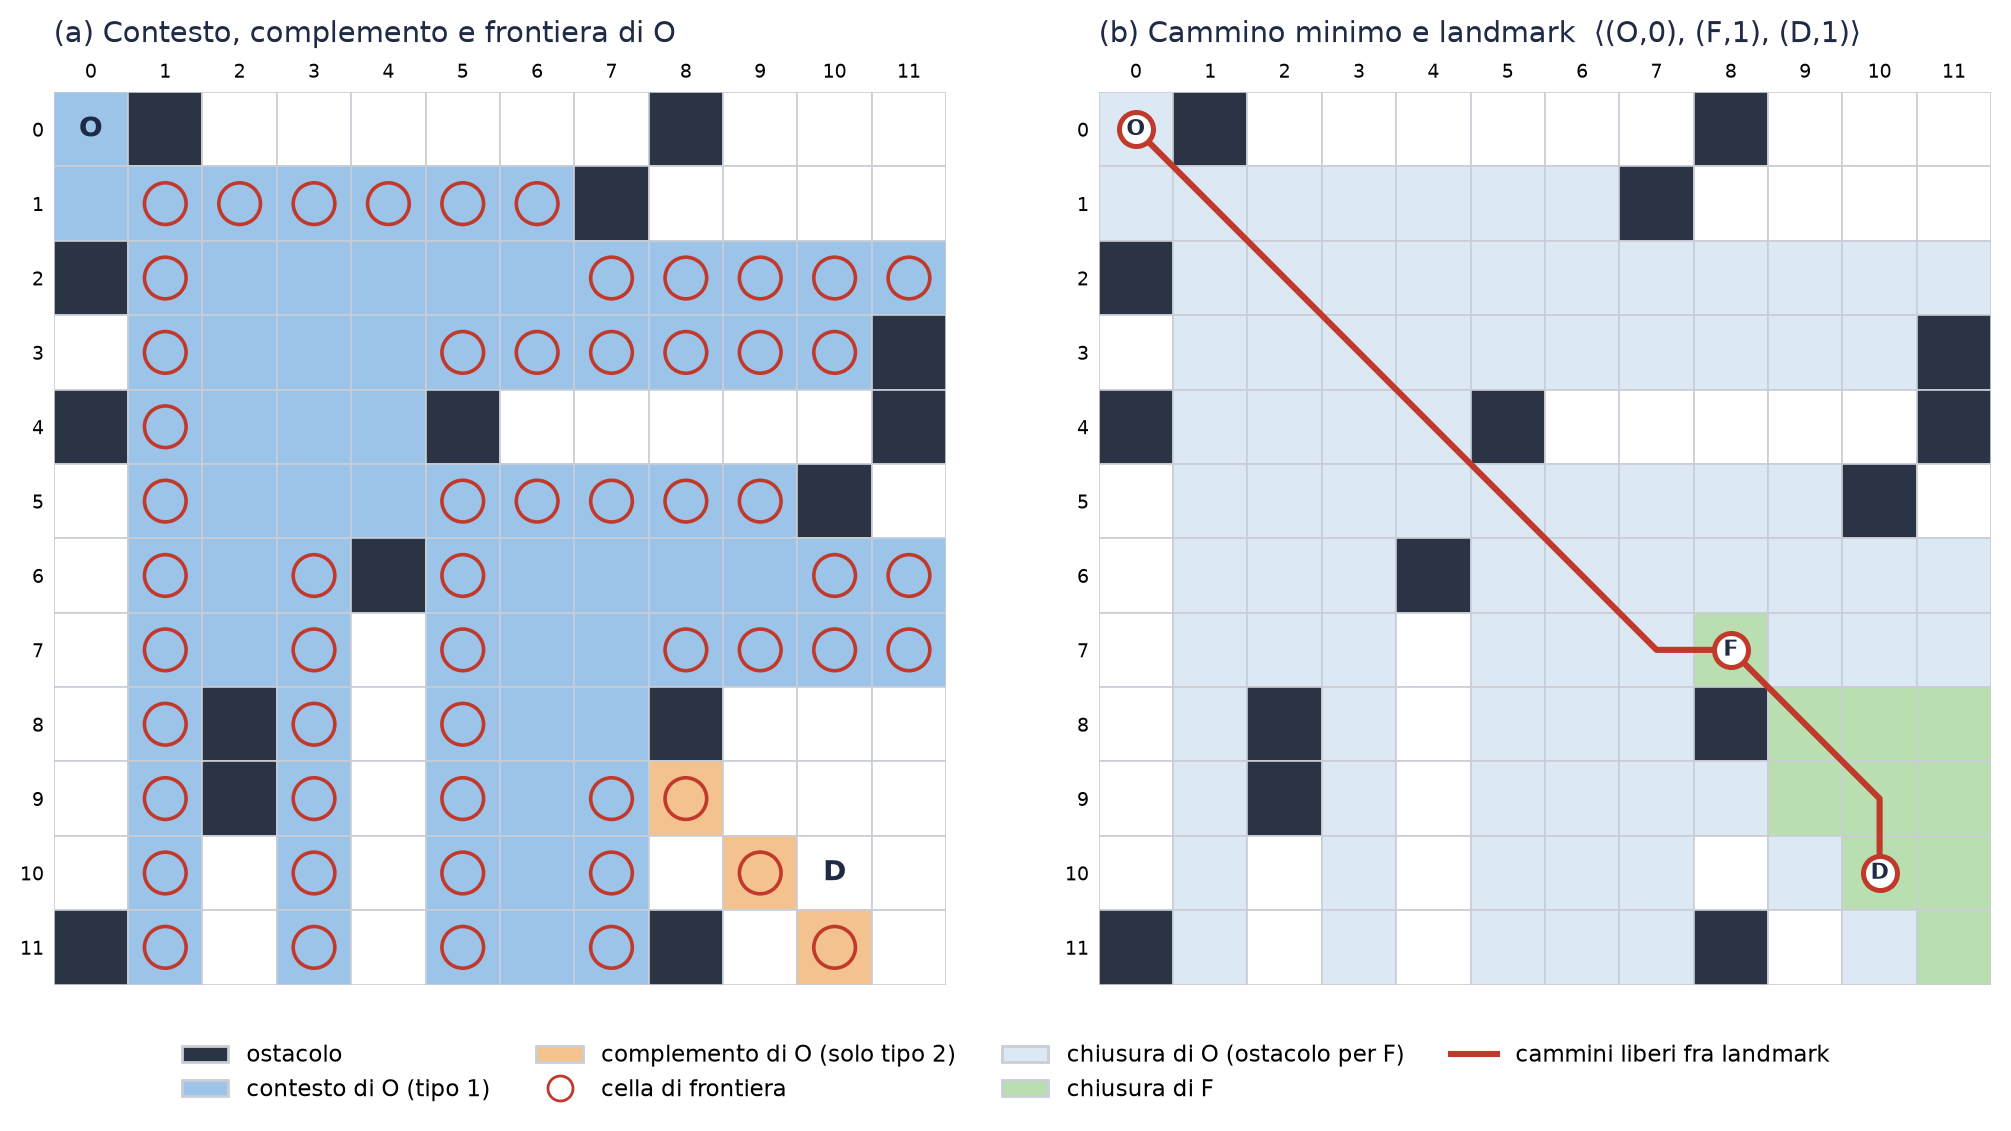
\includegraphics[width=\textwidth]{esempio_chiusura_landmark.png}
  \caption{Griglia $12\times 12$ con 15 ostacoli (seed 50), $O=(0,0)$ e
  $D=(10,10)$. (a) Contesto, complemento e frontiera di $O$ calcolati
  con l'\cref{alg:chiusura}. (b) Cammino minimo di lunghezza
  $9\sqrt{2}+2 \approx 14{,}728$ restituito da \cmin{}: $D$ non appartiene
  alla chiusura di $O$, quindi il cammino passa per la cella di frontiera
  $F=(8,7)$, la cui chiusura è calcolata trattando come ostacoli le celle
  della chiusura di $O$. I tratti fra landmark sono disegnati come cammini
  liberi a solo scopo illustrativo.}
  \label{fig:esempio}
\end{figure}

\begin{table}[H]
\centering
\small
\begin{tabular}{@{}r l l r@{}}
\toprule
\textbf{Valore} & \textbf{Bit} & \textbf{Proprietà} & \textbf{Celle} \\
\midrule
0   & \code{00000000} & libera, fuori dalla chiusura & 44 \\
1   & \code{00000001} & contesto                     & 22 \\
3   & \code{00000011} & contesto, regina             & 6 \\
5   & \code{00000101} & contesto, origine            & 1 \\
17  & \code{00010001} & contesto, frontiera          & 51 \\
19  & \code{00010011} & contesto, regina, frontiera  & 2 \\
24  & \code{00011000} & complemento, frontiera       & 3 \\
128 & \code{10000000} & ostacolo                     & 15 \\
\bottomrule
\end{tabular}
\caption{Stati delle celle nella griglia della \cref{fig:esempio}(a).}
\label{tab:stati-esempio}
\end{table}

\begin{algorithm}[H]
\caption{Calcolo di chiusura e frontiera di una cella $O$}
\label{alg:chiusura}
\begin{algorithmic}[1]
\Require griglia $g$ di dimensioni $W \times H$, cella $O$
\Ensure matrice degli stati $s$, chiusura di $O$, frontiera di $O$
\Procedure{CalcolaChiusura}{$g, O$}
  \State $s \gets$ matrice $H \times W$ con il solo bit \code{OSTACOLO} copiato da $g$
  \If{$O$ è un ostacolo} \Return $s, \emptyset, \emptyset$ \EndIf
  \ForEach{direzione primaria $d$ fra le otto}
    \ForEach{cella $c$ di \Call{Linea}{$g, O, d$}}
      \State $s[c] \gets s[c] \mathbin{|} \code{CONTESTO} \mathbin{|} \code{REGINA}$
      \State $\mathit{classe} \gets \code{CONTESTO}$ \textbf{if} $d$ è diagonale \textbf{else} $\code{COMPLEMENTO}$
      \ForEach{direzione laterale $\ell$ di $d$ (\cref{tab:direzioni})}
        \ForEach{cella $c'$ di \Call{Linea}{$g, c, \ell$}}
          \State $s[c'] \gets s[c'] \mathbin{|} \mathit{classe}$
        \EndFor
      \EndFor
    \EndFor
  \EndFor
  \ForEach{cella $c$ con $s[c]$ contenente \code{CONTESTO}}
    \State togli \code{COMPLEMENTO} da $s[c]$ \Comment{complemento esclusivo}
  \EndFor
  \State $s[O] \gets s[O] \mathbin{|} \code{ORIGINE} \mathbin{|} \code{CONTESTO}$
  \State $\mathit{chiusura} \gets \{c : s[c] \text{ contiene } \code{CONTESTO} \text{ o } \code{COMPLEMENTO}\}$
  \State $\mathit{frontiera} \gets \emptyset$
  \ForEach{$c \in \mathit{chiusura}$}
    \If{esiste un vicino $v$ di $c$ nella griglia, non ostacolo e non in $\mathit{chiusura}$}
      \State $s[c] \gets s[c] \mathbin{|} \code{FRONTIERA}$; \quad aggiungi $c$ a $\mathit{frontiera}$
    \EndIf
  \EndFor
  \State \Return $s, \mathit{chiusura}, \mathit{frontiera}$
\EndProcedure
\Statex
\Function{Linea}{$g, c, d$} \Comment{celle da $c$ (esclusa) in direzione $d$}
  \State $L \gets \seq{}$; \quad $c \gets c + d$
  \While{$c$ è nella griglia \textbf{and} $c$ non è un ostacolo}
    \State aggiungi $c$ a $L$; \quad $c \gets c + d$
  \EndWhile
  \State \Return $L$
\EndFunction
\end{algorithmic}
\end{algorithm}

\subsection{Frontiera}

Una cella della chiusura è di frontiera se almeno una delle otto celle
adiacenti è dentro la griglia, non è un ostacolo e non appartiene alla
chiusura. Le celle esterne alla griglia non contano come celle
attraversabili: se la chiusura copre tutta una griglia senza ostacoli, la
frontiera è vuota. Il tipo di una cella di frontiera si legge dal suo stato:
$t=1$ se ha il bit \code{CONTESTO}, $t=2$ altrimenti.

\subsection{Complessità}
\label{sec:complessita-chiusura}

Sia $n = WH$ il numero di celle.

\paragraph{Tempo.} La copia iniziale degli ostacoli, la passata che rende
esclusivo il complemento e la raccolta della chiusura scandiscono l'intera
griglia: $\Theta(n)$. Le linee primarie hanno lunghezza complessiva
$O(W+H)$. Le linee laterali che partono da una stessa linea primaria nella
stessa direzione sono parallele, quindi disgiunte; ogni cella può essere
attraversata al più da una laterale per ciascuna delle due linee primarie che
delimitano il suo ottante.
Le laterali visitano perciò $O(n)$ celle in totale. Il controllo della
frontiera esamina otto vicini per ogni cella della chiusura, $O(n)$.
Complessivamente il calcolo costa $\Theta(n)$, anche quando la chiusura è
piccola, perché le scansioni coprono sempre tutta la griglia.

\paragraph{Spazio.} La matrice degli stati occupa $4n$ byte (un \code{int}
per cella); la lista della chiusura e l'array della frontiera hanno al più
$n$ elementi. Lo spazio è quindi $\Theta(n)$.

Il costo lineare nella dimensione della griglia ha conseguenze sul Compito
Tre: \cmin{} calcola una chiusura a ogni chiamata ricorsiva non servita
dalla cache, quindi il suo costo è almeno proporzionale a $n$ per il numero
di chiusure calcolate (\cref{sec:analisi-teorica}).

\subsection{Applicazione}
\label{sec:applicazione-chiusura}

L'opzione \code{-{}-chiusura} esegue il solo Compito Due su una griglia
generata con i parametri della \cref{sec:compito1} oppure letta da un file
JSON prodotto dal generatore (\code{-{}-grid-input}). Per la cella $O$
indicata l'applicazione stampa la mappa della chiusura, il numero di celle di
contesto, complemento e frontiera, l'appartenenza di $D$ alla chiusura e la
distanza libera $\dlib(O,D)$, scomposta in mosse rettilinee e diagonali; con
\code{-{}-chiusura-output} salva anche gli stati di tutte le celle in JSON,
nel formato della \cref{tab:statocella}. Sulla griglia della
\cref{fig:esempio}(a) l'uscita è la seguente (le celle di frontiera
sono in maiuscolo) e i conteggi coincidono con la \cref{tab:stati-esempio}.

\begin{lstlisting}
java -jar asd-project.jar --grid-input risultati/griglie_json/scenario_02_12x12_15ost_seed50.json --origin 0,0 --destination 10,10 --chiusura
O   #   .   .   .   .   .   .   #   .   .   .
c   C   C   C   C   C   C   #   .   .   .   .
#   C   c   c   c   c   c   C   C   C   C   C
.   C   c   c   c   C   C   C   C   C   C   #
#   C   c   c   c   #   .   .   .   .   .   #
.   C   c   c   c   C   C   C   C   C   #   .
.   C   c   C   #   C   c   c   c   c   C   C
.   C   c   C   .   C   c   c   C   C   C   C
.   C   #   C   .   C   c   c   #   .   .   .
.   C   #   C   .   C   c   C   K   .   .   .
.   C   .   C   .   C   c   C   .   K   D   .
#   C   .   C   .   C   c   C   #   .   K   .
Legenda: O origine, D destinazione, # ostacolo, c contesto (tipo 1), k complemento (tipo 2), maiuscole = frontiera, . fuori dalla chiusura
Contesto: 82 celle | complemento: 3 celle | frontiera: 56 celle (53 di tipo 1, 3 di tipo 2)
O=(0,0), D=(10,10): D si trova fuori dalla chiusura di O
dlib(O,D) = 0 + 10*sqrt(2) = 14.142136 (0 mosse rettilinee, 10 diagonali)
\end{lstlisting}

\subsection{Verifica}

Oltre ai test unitari su casi costruiti a mano, \code{CalcoloChiusura} è
confrontato con un \emph{oracolo}, cioè un'implementazione di riferimento che
calcola lo stesso risultato con un metodo diverso e più semplice, così che un
errore difficilmente sia comune ai due. L'oracolo
(\code{CalcoloChiusuraOracleTest}) non usa linee primarie e laterali: per ogni
cella $c$ percorre l'unico cammino di tipo~1 e l'unico di tipo~2 da $O$ a $c$
e controlla che non attraversino ostacoli, applicando direttamente la
definizione; la frontiera è ricavata dalla chiusura così ottenuta. Il test
enumera tutte le $2^9 = 512$ disposizioni di ostacoli su una griglia
$3\times3$ e, per ogni origine libera, richiede che contesto, complemento,
chiusura e frontiera coincidano cella per cella. Un test dedicato verifica che la mossa
diagonale fra due ostacoli adiacenti per uno spigolo sia ammessa e costi
$\sqrt{2}$.
\clearpage
\section{Compito Tre: l'algoritmo CamminoMin}
\label{sec:compito3}

\subsection{Idea e pseudocodice di riferimento}

Se $D$ appartiene alla chiusura di $O$, un cammino minimo è il cammino libero
fra le due celle e la sua lunghezza è $\dlib(O,D)$. Altrimenti, qualunque
cammino da $O$ a $D$ esce dalla chiusura di $O$ passando per una cella della
sua frontiera. La traccia definisce quindi ricorsivamente il cammino minimo
come il più corto fra i cammini ottenuti componendo il cammino libero da $O$
a una cella di frontiera $F$ con un cammino minimo da $F$ a $D$, al variare di
$F$ nella frontiera. Nella chiamata su $F$ le celle della chiusura di $O$
sono trattate come ostacoli, così il cammino non ripassa da una regione già
coperta.

L'\cref{alg:traccia} riporta lo pseudocodice della traccia (pag.~30); la
numerazione delle righe è quella usata nel resto della relazione.

\begin{algorithm}[H]
\caption{\cmin{} come definito nella traccia~\cite{traccia}}
\label{alg:traccia}
\begin{algorithmic}[1]
\Procedure{CamminoMin}{$O, D, \mathit{dim}, \mathit{osta}$}
  \LineComment{$\mathit{dim}$: dimensioni della griglia; $\mathit{osta}$: celle non attraversabili}
  \State $\mathit{contesto} \gets \Call{CalcolaContesto}{O, \mathit{dim}, \mathit{osta}}$
  \If{$D \in \mathit{contesto}$}
    \State \Return $\dlib(O,D), \seq{(O,0), (D,1)}$
  \EndIf
  \State $\mathit{complemento} \gets \Call{CalcolaComplemento}{O, \mathit{dim}, \mathit{osta}}$
  \If{$D \in \mathit{complemento}$}
    \State \Return $\dlib(O,D), \seq{(O,0), (D,2)}$
  \EndIf
  \State $\mathit{frontiera} \gets \Call{CalcolaFrontiera}{\mathit{contesto}, \mathit{complemento}, \mathit{dim}, \mathit{osta}}$
  \If{$\mathit{frontiera} = \emptyset$} \Comment{vicolo cieco}
    \State \Return $\infty, \seq{}$
  \EndIf
  \State $\mathit{lunghezzaMin} \gets \infty$
  \State $\mathit{seqMin} \gets \seq{}$
  \ForEach{$(F,t) \in \mathit{frontiera}$}
    \State $\mathit{lF} \gets \dlib(O,F)$
    \If{$\mathit{lF} < \mathit{lunghezzaMin}$}
      \LineComment{una condizione più forte è $\mathit{lF} + \dlib(F,D) < \mathit{lunghezzaMin}$}
      \State $\mathit{lFD}, \mathit{seqFD} \gets \Call{CamminoMin}{F, D, \mathit{dim}, \mathit{osta} \cup \mathit{contesto} \cup \mathit{complemento}}$
      \State $\mathit{lTot} \gets \mathit{lF} + \mathit{lFD}$
      \If{$\mathit{lTot} < \mathit{lunghezzaMin}$}
        \State $\mathit{lunghezzaMin} \gets \mathit{lTot}$
        \State $\mathit{seqMin} \gets \Call{Compatta}{\seq{(O,0),(F,t)}, \mathit{seqFD}}$
      \EndIf
    \EndIf
  \EndFor
  \State \Return $\mathit{lunghezzaMin}, \mathit{seqMin}$
\EndProcedure
\end{algorithmic}
\end{algorithm}

\subsection{Implementazione}
\label{sec:implementazione-cmin}

La classe \code{CamminoMin} implementa l'\cref{alg:impl}. Il metodo
pubblico \code{calcola(griglia, O, D)} restituisce un
\code{Cammino}, formato dalla lunghezza (\code{DistanzaLibera}) e dalla lista
dei landmark. Due sovraccarichi ricevono anche un oggetto
\code{StatisticheEsecuzione}, in cui accumulare i contatori del riassunto, e la
variante dell'algoritmo da eseguire (\cref{sec:varianti}); senza indicazioni
si usa la variante \code{base}.

\begin{algorithm}[tbp]
\caption{\cmin{} come implementato in \code{CamminoMin}}
\label{alg:impl}
\begin{algorithmic}[1]
\Require griglia $g$, celle attraversabili $O$ e $D$, limite $L$ ($\infty$ nella chiamata principale), tabella $\mathit{cache}$ (vuota alla prima chiamata)
\Ensure lunghezza del cammino minimo da $O$ a $D$ e sequenza dei landmark, oppure $(\infty, \seq{})$ se non esiste un cammino più corto di $L$
\Function{CamminoMin}{$g, O, D, L$}
  \State $k \gets \Call{Chiave}{\text{ostacoli di } g, O, D}$
  \If{$\mathit{cache}[k]$ è esatto, o esclude cammini più corti di un $L' \ge L$}
    \State \Return $\mathit{cache}[k]$ \Comment{$(\infty, \seq{})$ nel secondo caso}
  \EndIf
  \State $s, \mathit{chiusura}, \mathit{frontiera} \gets \Call{CalcolaChiusura}{g, O}$ \Comment{\cref{alg:chiusura}}
  \If{$s[D]$ contiene \code{CHIUSURA}} \Comment{righe 4--8, anche $O = D$}
    \State $r \gets \bigl(\dlib(O,D), \seq{(O,0), (D, \Call{Tipo}{s[D]})}\bigr)$
    \State $\mathit{cache}[k] \gets r$ (esatto); \quad \Return $r$
  \EndIf
  \State $\mathit{lunghezzaMin} \gets L$; \quad $\mathit{seqMin} \gets \seq{}$
  \State ordina $\mathit{frontiera}$ per $\dlib(O,F) + \dlib(F,D)$ crescente
  \ForEach{$F \in \mathit{frontiera}$}
    \State $\mathit{lF} \gets \dlib(O,F)$
    \If{$\mathit{lF} \ge \mathit{lunghezzaMin}$} \Continue \Comment{riga 16 falsa}
    \EndIf
    \If{$\mathit{lF} + \dlib(F,D) \ge \mathit{lunghezzaMin}$} \Continue \Comment{riga 17 falsa}
    \EndIf
    \State $g' \gets g$ con le celle di $\mathit{chiusura} \setminus \{F\}$ come ostacoli
    \State $L' \gets \mathit{lunghezzaMin} - \mathit{lF}$ se il limite è propagato, altrimenti $\infty$
    \State $\mathit{lFD}, \mathit{seqFD} \gets \Call{CamminoMin}{g', F, D, L'}$
    \If{$\mathit{lF} + \mathit{lFD} < \mathit{lunghezzaMin}$}
      \State $\mathit{lunghezzaMin} \gets \mathit{lF} + \mathit{lFD}$
      \State $\mathit{seqMin} \gets \seq{(O,0), (F, \Call{Tipo}{s[F]})} \cdot \mathit{seqFD}[2..]$ \Comment{\textsc{Compatta}}
    \EndIf
  \EndFor
  \If{$\mathit{seqMin} = \seq{}$} \Comment{nessun cammino più corto di $L$}
    \State $\mathit{cache}[k] \gets$ ``nessun cammino più corto di $L$''; \quad \Return $(\infty, \seq{})$
  \EndIf
  \State $\mathit{cache}[k] \gets (\mathit{lunghezzaMin}, \mathit{seqMin})$ (esatto)
  \State \Return $\mathit{lunghezzaMin}, \mathit{seqMin}$
\EndFunction
\end{algorithmic}
\end{algorithm}

Senza limite propagato $L$ vale sempre $\infty$ e l'algoritmo coincide con la
versione della traccia arricchita da ordinamento, riga~17 e cache.

La \cref{tab:corrispondenza} collega le righe della traccia
all'implementazione. La traccia ammette una codifica diversa dallo
pseudocodice purché produca gli stessi effetti (pag.~34--35).

\begin{table}[H]
\centering
\small
\begin{tabularx}{\textwidth}{@{}l X@{}}
\toprule
\textbf{Righe della traccia} & \textbf{Implementazione} \\
\midrule
3, 6, 9  & Un'unica chiamata a \code{CalcoloChiusura} produce contesto,
           complemento, frontiera e tipo di ogni cella (\cref{sec:chiusura}). \\
4--8     & Il caso base controlla la maschera \code{CHIUSURA} nello stato di
           $D$; il tipo di $D$ è $1$ se ha il bit \code{CONTESTO}, $2$
           altrimenti. Se $O = D$, $O$ è nel proprio contesto e il risultato è
           $\bigl(0, \seq{(O,0),(O,1)}\bigr)$, come richiesto a pag.~32. \\
10--11   & Con frontiera vuota il ciclo non esegue iterazioni e la funzione
           restituisce $(\infty, \seq{})$, cioè lo stesso risultato. \\
12--13   & $\mathit{lunghezzaMin}$ parte da $\infty$, oppure dal limite
           ricevuto se il limite è propagato (\cref{sec:ottimizzazioni}). \\
14       & La frontiera è visitata in ordine di limite inferiore crescente.
           $O$ non è mai di frontiera: i suoi vicini attraversabili sono le
           prime celle delle linee primarie e appartengono al contesto. \\
16--17   & La condizione della riga 16 è controllata per prima, poi quella
           più forte suggerita alla riga 17. I due esiti negativi sono
           contati separatamente (\cref{sec:contatori}). \\
18       & Gli ostacoli della chiamata ricorsiva sono quelli di $g$ più la
           chiusura di $O$ tranne $F$ (\cref{sec:ostacoli-annidati}). \\
20--22   & Il confronto è stretto: a parità di lunghezza resta il primo
           cammino trovato. \textsc{Compatta} sostituisce il primo landmark
           $(F,0)$ di $\mathit{seqFD}$ con $(F,t)$. \\
\bottomrule
\end{tabularx}
\caption{Corrispondenza fra lo pseudocodice della traccia e l'implementazione.}
\label{tab:corrispondenza}
\end{table}

\subsection{Ostacoli nelle chiamate annidate}
\label{sec:ostacoli-annidati}

Secondo la traccia (pag.~28 e 32), nella chiamata su $F$ tutte le celle della
chiusura di $O$ diventano ostacoli, compresa $F$, che però resta l'origine
della nuova chiusura. L'implementazione ottiene lo stesso effetto escludendo
$F$ dall'insieme di ostacoli aggiunti: le celle raggiungibili da $F$ sono le
stesse, e \code{CalcoloChiusura} non deve gestire un'origine marcata come
ostacolo. La nuova griglia $g'$ è una vista immutabile
(\cref{sec:immutabilita}): ogni ramo ricorsivo accumula i propri ostacoli
senza modificare la griglia dei rami fratelli.

\subsection{Sequenza dei landmark}

La sequenza dei landmark $\seq{(O,0), (F_1,t_1), \dots, (D,t_D)}$ elenca
l'origine e le celle di frontiera attraversate dal cammino; il tipo di un
landmark è quello del cammino libero che lo raggiunge dal landmark
precedente, quindi la sequenza descrive il cammino in modo univoco.
Nell'implementazione un landmark è un record con le coordinate e il tipo
$t \in \{0, 1, 2\}$; il tipo $0$ identifica l'origine della chiamata. La
lista dei landmark di un \code{Cammino} è immutabile. Se $D$ è
irraggiungibile il risultato è la lunghezza infinita con la sequenza vuota.

Nell'esempio della \cref{fig:esempio}(b) la chiamata da $O=(0,0)$ restituisce
$\seq{(O,0), ((8,7),1), (D,1)}$. La chiamata nel verso opposto, da
$(10,10)$ a $(0,0)$, restituisce
$\seq{((10,10),0), ((0,1),2), ((0,0),1)}$: un cammino diverso, ma della stessa
lunghezza $9\sqrt{2}+2$. In entrambi i casi la somma delle distanze libere
fra landmark consecutivi è uguale alla lunghezza del cammino; i test
verificano questa proprietà su tutti i risultati finiti.

\subsection{Ottimizzazioni}
\label{sec:ottimizzazioni}

Le ottimizzazioni riducono il numero di chiamate ricorsive senza cambiare la
lunghezza restituita; il loro effetto è misurato nella \cref{sec:ablation}.

\paragraph{Ordinamento della frontiera.} Le celle di frontiera sono visitate
in ordine crescente di $\dlib(O,F) + \dlib(F,D)$, un limite inferiore della
lunghezza di qualunque cammino da $O$ a $D$ che passi per $F$. I candidati
più promettenti vengono esplorati per primi, $\mathit{lunghezzaMin}$ scende
presto e le condizioni di potatura scartano più rami. L'ordinamento costa
$O(f \log f)$, con $f$ numero di celle di frontiera; le due distanze libere di
ogni candidato sono calcolate una volta sola e riusate dalla potatura.

\paragraph{Condizione della riga 17.} Dopo la riga 16 viene controllata la
condizione più forte $\mathit{lF} + \dlib(F,D) < \mathit{lunghezzaMin}$. La
potatura è corretta perché $\dlib(F,D)$ non supera la lunghezza di nessun
cammino da $F$ a $D$: se la condizione è falsa, passare per $F$ non può dare
un cammino strettamente più corto di quello già trovato. Il confronto
sperimentale fra le due condizioni, facoltativo per i gruppi di tre persone
(pag.~67), non fa parte di questo progetto.

\paragraph{Memoizzazione.} Il risultato di una chiamata dipende dagli
ostacoli della griglia, da $O$, da $D$ e, con il limite propagato, dal limite
ricevuto. Il risultato viene salvato in una \code{HashMap} la cui chiave è
formata dal \code{BitSet} degli ostacoli della vista (\cref{sec:immutabilita})
e dalle coordinate di $O$ e $D$: la chiave occupa $n/8$ byte e
\code{equals} e \code{hashCode} costano $O(n/64)$. La chiave è esatta, perché
un hash intero degli ostacoli potrebbe collidere e restituire il risultato di
un altro sottoproblema. Una prima versione usava una stringa con le
coordinate di tutti gli ostacoli: chiavi equivalenti, ma costruite con una
scansione della griglia e lunghe decine di caratteri per ostacolo. Le
direzioni $O \to D$ e $D \to O$ usano tabelle separate, così la verifica di
simmetria confronta due calcoli indipendenti.

\paragraph{Limite propagato.} Nella versione della traccia ogni chiamata
annidata cerca il cammino minimo da $F$ a $D$ partendo da
$\mathit{lunghezzaMin} = \infty$, anche quando il chiamante ha già un cammino
di lunghezza $\mathit{lunghezzaMin}$ e gli serve soltanto sapere se ne esiste
uno più corto di $\mathit{lunghezzaMin} - \dlib(O,F)$. La variante con limite
propagato passa questo valore $L'$ alla chiamata annidata, che inizializza
con esso il proprio $\mathit{lunghezzaMin}$: le righe 16 e 17 potano così
anche all'interno della ricorsione. Una chiamata con limite $L$ restituisce
il cammino minimo del sottoproblema se è più corto di $L$, altrimenti
$(\infty, \seq{})$. Il risultato resta corretto: un cammino trovato sotto il
limite viene confrontato con tutti i candidati che potrebbero batterlo, ed è
quindi il minimo; un ramo che non trova nulla sotto il limite non può
migliorare il cammino del chiamante. La cache distingue i due casi: un
risultato trovato è esatto e vale per qualunque limite; un risultato vuoto
significa soltanto ``nessun cammino più corto di $L$'' e viene riusato solo
per chiamate con limite non superiore a $L$.

\paragraph{Viste immutabili.} La griglia $g'$ della chiamata ricorsiva
richiede la copia di un \code{BitSet} di $n$ bit e l'inserimento delle celle
della chiusura, invece della copia di una matrice di $n$ interi.

\subsection{Varianti}
\label{sec:varianti}

L'enumerazione \code{VarianteCamminoMin} attiva o disattiva le
ottimizzazioni, per confrontarle nella sperimentazione
(\cref{tab:varianti}). La riga~17 è attiva in tutte le varianti. La variante
si sceglie da riga di comando con \code{-{}-variante}.

\begin{table}[H]
\centering
\small
\begin{tabular}{@{}l c c c@{}}
\toprule
\textbf{Variante} & \textbf{Cache} & \textbf{Ordinamento} & \textbf{Limite propagato} \\
\midrule
\code{base}              & sì & sì & no \\
\code{senza-cache}       & no & sì & no \\
\code{senza-ordinamento} & sì & no, ordine di scansione della griglia & no \\
\code{limite-propagato}  & sì & sì & sì \\
\bottomrule
\end{tabular}
\caption{Varianti di \cmin{}. Tutte restituiscono la stessa lunghezza minima.}
\label{tab:varianti}
\end{table}

\subsection{Contatori e riassunto}
\label{sec:contatori}

La traccia chiede, per ogni istanza e su richiesta dell'utente, un riassunto
con dimensioni e tipo della griglia, numero totale di celle di frontiera,
numero di volte in cui la condizione della riga 16/17 è risultata falsa e
prestazioni (pag.~71). \code{StatisticheEsecuzione} raccoglie i contatori
della \cref{tab:contatori} durante l'esecuzione. Un'istanza comprende sempre
entrambe le direzioni $O \to D$ e $D \to O$; i contatori sommano le due
direzioni e tutte le chiamate ricorsive.

\begin{table}[H]
\centering
\small
\begin{tabularx}{\textwidth}{@{}l X@{}}
\toprule
\textbf{Campo} & \textbf{Significato} \\
\midrule
\code{front}         & celle di frontiera di tutte le chiusure calcolate
                       (le chiamate servite dalla cache non calcolano chiusure) \\
\code{r16False}      & volte in cui la condizione della riga 16 è risultata falsa \\
\code{r17Prune}      & volte in cui la riga 16 era vera ma la condizione più forte
                       della riga 17 era falsa \\
\code{pruneTot}      & somma dei due precedenti: volte in cui la condizione
                       effettivamente usata è risultata falsa e il ramo è stato potato \\
\code{variante}      & variante di \cmin{} eseguita (\cref{tab:varianti}) \\
\code{chiamate}      & invocazioni di \cmin{}, comprese quelle servite dalla cache \\
\code{cacheHit}      & invocazioni servite dalla cache, che non calcolano una chiusura \\
\code{prof}          & profondità massima della ricorsione \\
\code{chiusurePicco} & massimo numero di matrici di chiusura presenti
                       contemporaneamente in memoria \\
\code{memEst}        & stima della memoria di tali matrici:
                       $\code{chiusurePicco} \cdot 4n$ byte \\
\code{tempoNs}       & tempo minimo, mediano e massimo delle ripetizioni (\cref{sec:protocollo}) \\
\code{seqOD}, \code{seqDO} & sequenze dei landmark nei due versi \\
\bottomrule
\end{tabularx}
\caption{Contatori del riassunto. L'elenco completo delle colonne del CSV è
nell'\cref{app:formato}.}
\label{tab:contatori}
\end{table}

Poiché $\dlib(F,D) \ge 0$, quando la condizione della riga 16 è falsa lo è
anche quella della riga 17. \code{pruneTot} conta quindi le volte in cui la
condizione della riga 17 è risultata falsa, e \code{r16False} quante di
queste sarebbero state potate anche dalla sola riga 16. La profondità e le
chiusure presenti in memoria possono differire: una chiamata servita dalla
cache aumenta la profondità ma non alloca una nuova matrice.

Il riassunto viene stampato su una riga per istanza e variante, con le
lunghezze arrotondate a quattro decimali; nel piano sperimentale i riassunti
sono salvati anche in \code{risultati/riassunti.txt}. Per un'istanza singola
l'opzione \code{-{}-summary false} omette la stampa, mentre il CSV contiene
sempre tutti i campi, con sei decimali. Il riassunto dell'istanza della \cref{fig:esempio} nel piano
sperimentale è:

\begin{lstlisting}
[G12x12_d10_s50_p1] variante=base | tipo=Casuale | 12x12 | ost=15 | O=(0,0)->D=(10,10) | OD=14.7279 | DO=14.7279 | corr=true | front=118 | r16False=1 | r17Prune=96 | pruneTot=97 | chiamate=18 | cacheHit=2 | prof=4 | chiusurePicco=4 | memEst=2304B | tempoNs[min/med/max]=180900/184000/218900 | warmup=1 | rip=5 | seqOD=[(x=0,y=0,tipo=0), (x=8,y=7,tipo=1), (x=10,y=10,tipo=1)] | seqDO=[(x=10,y=10,tipo=0), (x=0,y=1,tipo=2), (x=0,y=0,tipo=1)]
\end{lstlisting}
\clearpage
\section{Compito Quattro: analisi e sperimentazione}
\label{sec:compito4}

\subsection{Analisi teorica}
\label{sec:analisi-teorica}

Nel seguito $n = WH$ è il numero di celle della griglia, $C$ il numero
totale di invocazioni di \cmin{} (comprese quelle servite dalla cache),
$C_c \le C$ il numero di invocazioni che calcolano una chiusura, $f_i$ il
numero di celle di frontiera dell'invocazione $i$ e $l$ la profondità
massima della ricorsione.

\paragraph{Tempo di una invocazione.} Un'invocazione cerca il proprio
sottoproblema nella cache: la chiave riusa il \code{BitSet} degli ostacoli
della vista, quindi \code{hashCode} ed \code{equals} costano $O(n/64)$. Se la
chiave è presente si ferma. Altrimenti calcola la chiusura, $\Theta(n)$
(\cref{sec:complessita-chiusura}), e ordina la frontiera,
$O(f_i \log f_i)$. Per ogni cella di frontiera non potata costruisce la
griglia della chiamata ricorsiva, $O(n)$; questo costo si può attribuire
all'invocazione figlia. Poiché $f_i \le n$, il tempo totale è
\begin{equation}
  T = \sum_{i=1}^{C_c} O(n + f_i \log f_i) + O(C \cdot n/64)
    = O(C_c \cdot n \log n + C \cdot n),
  \qquad T = \Omega(C_c \cdot n).
  \label{eq:tempo}
\end{equation}
Il prodotto $C_c \cdot n$, chiamato \emph{lavoro stimato} nel seguito, è
quindi la grandezza che dovrebbe guidare il tempo misurato.

\paragraph{Caso migliore.} Se $D$ appartiene alla chiusura di $O$ basta una
invocazione per verso e il costo è $\Theta(n)$. È il caso di 28 delle 67
istanze del piano sperimentale; in una ventinovesima, sulla griglia
$5\times5$ quasi piena, la frontiera di $O$ è vuota e il risultato $\infty$
si ottiene ugualmente con una sola invocazione per verso.

\paragraph{Caso peggiore.} Ogni chiamata annidata aggiunge agli ostacoli
almeno la cella da cui parte la chiusura precedente, quindi lungo un ramo il
numero di celle libere diminuisce strettamente e $l \le n$. Ogni invocazione
ha al più $f_i \le n$ figli. Il numero di invocazioni è quindi limitato da
una quantità esponenziale, dell'ordine di $n^{l}$; questa analisi non fornisce
un limite polinomiale in $n$, e la sperimentazione mostra una crescita
combinatoria. Ordinamento della frontiera, potatura, cache e limite
propagato riducono $C$ in pratica ma non cambiano il caso peggiore. Nel piano,
con la variante \code{base}, $C$ arriva a \num{102202} su una griglia di 400
celle (\num{435793} senza cache) e nella serie sui limiti di scala a
\num{508161} (\cref{sec:limiti-scala}).

\paragraph{Spazio.} Ogni invocazione attiva che non è servita dalla cache
tiene in memoria la propria matrice degli stati ($4n$ byte), la chiusura e
la frontiera ($O(n)$) e la griglia del figlio in esecuzione ($n$ bit). La
pila delle chiamate occupa quindi $O(l \cdot n)$. La cache conserva un
elemento per ogni sottoproblema risolto: la chiave contiene un
\code{BitSet} di $n$ bit e il valore una sequenza di al più $l+1$ landmark.
Lo spazio totale è
\begin{equation}
  S = O(l \cdot n) + O\bigl(C_c \cdot (n/8 + l)\bigr) \text{ byte},
  \label{eq:spazio}
\end{equation}
dominato dalla cache quando $C_c$ cresce. La stima \code{memEst} del
riassunto conta soltanto le matrici della pila
($\code{chiusurePicco} \cdot 4n$ byte) e va letta come limite inferiore
della memoria effettivamente usata.

\subsection{Piano sperimentale e protocollo}
\label{sec:protocollo}

Il piano comprende 23 griglie casuali e 67 istanze, cioè coppie $(O,D)$
(\cref{tab:piano}). Le dimensioni vanno da $12\times12$ a $50\times50$; per
ogni dimensione c'è una griglia senza ostacoli, che isola il costo del caso
base, e le griglie con ostacoli sono generate da seed consecutivi. Il peso
del piano è sulle griglie $20\times20$ con densità fra il 5\% e il 20\%, dove
la ricorsione è significativa ma ogni variante termina in tempi brevi. Le
istanze più difficili sono coperte dalla serie sui limiti di scala
(\cref{sec:limiti-scala}).

Ogni istanza viene eseguita con più varianti di \cmin{}
(\cref{tab:varianti}). Le griglie senza ostacoli e il caso irraggiungibile
usano solo \code{base} e \code{limite-propagato}, perché basta una chiamata
per verso. Le griglie con ostacoli usano anche \code{senza-cache} e, dove
termina in tempi accettabili, \code{senza-ordinamento}. In prove
preliminari, sulle griglie $20\times20$ al 20\% una sola esecuzione senza
ordinamento richiedeva da alcuni secondi a qualche decina di secondi e
milioni di chiamate: per
mantenere il piano entro pochi minuti la variante è stata esclusa da quel
gruppo e dalle griglie $30\times30$ e $50\times50$. In totale il piano
comprende 215 esecuzioni (istanza e variante).

\begin{table}[H]
\centering
\small
\begin{tabular}{@{}l r r l r r l@{}}
\toprule
\textbf{Dimensione} & \textbf{Ostacoli} & \textbf{Densità} & \textbf{Seed} & \textbf{Griglie} & \textbf{Istanze} & \textbf{Varianti} \\
\midrule
$12\times12$ & 0  & 0\%    & 50        & 1 & 3 & B, L \\
$12\times12$ & 15 & 10,4\% & 50--52    & 3 & 9 & tutte \\
$20\times20$ & 0  & 0\%    & 100       & 1 & 3 & B, L \\
$20\times20$ & 20 & 5\%    & 100--102  & 3 & 9 & tutte \\
$20\times20$ & 40 & 10\%   & 100--102  & 3 & 9 & tutte \\
$20\times20$ & 80 & 20\%   & 100--102  & 3 & 9 & B, C, L \\
$30\times30$ & 0  & 0\%    & 200       & 1 & 3 & B, L \\
$30\times30$ & 45 & 5\%    & 200--202  & 3 & 9 & B, C, L \\
$50\times50$ & 0  & 0\%    & 300       & 1 & 3 & B, L \\
$50\times50$ & 50 & 2\%    & 300--302  & 3 & 9 & B, C, L \\
$5\times5$   & 23 & 92\%   & 1         & 1 & 1 & B, L \\
\midrule
\textbf{Totale} & & & & \textbf{23} & \textbf{67} & \\
\bottomrule
\end{tabular}
\caption{Griglie e istanze del piano sperimentale. Varianti: B = \code{base},
C = \code{senza-cache}, L = \code{limite-propagato}; ``tutte'' comprende
anche \code{senza-ordinamento}.}
\label{tab:piano}
\end{table}

Su ogni griglia si provano tre coppie, definite come frazioni delle
coordinate massime: dall'angolo in alto a sinistra a quello in basso a destra
(5\% $\to$ 95\%), dall'angolo in alto a destra a quello in basso a sinistra,
e dal centro verso l'alto a destra (50\% $\to$ (90\%, 10\%)). Se la cella
indicata è un ostacolo si usa la cella libera più vicina in distanza di
Chebyshev. La griglia $5\times5$ con 23 ostacoli ha una sola coppia, scelta
in modo che $D$ sia irraggiungibile, per verificare il risultato
$(\infty, \seq{})$ anche nel piano e non solo nei test.

Prima delle misure l'intero piano viene eseguito una volta, senza
registrare i tempi, per completare la compilazione JIT della JVM. Poi, per
ogni istanza e variante:

\begin{enumerate}
  \item si esegue una ripetizione di riscaldamento, esclusa dalle misure;
  \item seguono 5 ripetizioni misurate; ciascuna misura con
        \code{System.nanoTime()} il tempo complessivo di
        $\cmin(O,D)$ e $\cmin(D,O)$;
  \item il tempo dell'esecuzione è la mediana delle 5 misure; si registrano
        anche minimo e massimo;
  \item i contatori, che non dipendono dal tempo, devono coincidere in tutte
        le ripetizioni, altrimenti l'esecuzione si interrompe con un errore;
        si conservano quelli della ripetizione mediana.
\end{enumerate}

Le misure sono state raccolte l'8 novembre 2026 su un AMD Ryzen 7 5800X (8
core, 16 thread) con 31,9 GiB di RAM, Windows 11 Pro e Eclipse Temurin
21.0.6. L'algoritmo è sequenziale e usa un solo thread. Il piano completo,
compreso il passaggio di riscaldamento, richiede meno di un minuto.

\subsection{Verifica della correttezza}
\label{sec:verifica-cmin}

\paragraph{Simmetria e coerenza fra varianti.} Per ogni istanza la traccia
chiede di confrontare le lunghezze calcolate nei due versi. Tutte le 215
esecuzioni superano il controllo: 66 istanze hanno lunghezze finite che
differiscono meno di $10^{-10}$, l'istanza $5\times5$ ha lunghezza infinita
e sequenza vuota in entrambi i versi. Lo script di analisi verifica inoltre
che su ogni istanza tutte le varianti eseguite restituiscano la stessa
lunghezza. Le sequenze dei landmark nei due versi sono in generale diverse,
come nell'esempio della \cref{fig:esempio}.

\paragraph{Oracolo indipendente.} La simmetria non rileva un errore che
colpisca allo stesso modo entrambi i versi. Per questo un test confronta
\cmin{}, in tutte e quattro le varianti, con l'algoritmo di
Dijkstra~\cite{dijkstra} sul grafo delle celle libere, con archi di costo
$1$ e $\sqrt{2}$. Le istanze sono 500 griglie $5\times5$ con 0--20 ostacoli
e coppie $(O,D)$ estratte a caso da un seed fisso. Il test richiede che:

\begin{itemize}
  \item le due lunghezze coincidano, oppure siano entrambe infinite con
        sequenza vuota;
  \item la sequenza dei landmark inizi con $(O,0)$, termini in $D$ e abbia
        tipi $1$ o $2$ su celle libere;
  \item per ogni coppia di landmark consecutivi la distanza libera coincida
        con la distanza di Dijkstra sulla griglia originale, cioè il tratto
        sia realizzabile come cammino libero;
  \item la somma dei tratti sia uguale alla lunghezza restituita.
\end{itemize}

\paragraph{Griglie strutturate.} Le griglie $5\times5$ producono ricorsioni
poco profonde. Altri tre test applicano lo stesso confronto con Dijkstra, in
entrambi i versi e per tutte le varianti, a griglie in cui il cammino deve
attraversare molti landmark:

\begin{itemize}
  \item una \emph{serpentina} $15\times15$, con muri orizzontali e varchi
        alternati a destra e a sinistra: il cammino ha 8 landmark e la
        ricorsione arriva a profondità 8 con 90 chiamate, 46 delle quali
        servite dalla cache;
  \item una \emph{spirale} $13\times13$ con un corridoio largo una cella:
        13 landmark e profondità 12;
  \item 50 griglie casuali $10\times10$ con il 20\% di ostacoli.
\end{itemize}

\paragraph{Regressione.} Un test fissa i contatori della variante
\code{base} sull'istanza della \cref{fig:esempio}, un altro verifica che il
generatore produca le stesse griglie di un'implementazione di riferimento
che aggiunge gli ostacoli uno alla volta, e un terzo
che il limite propagato riduca le chiamate senza cambiare la lunghezza
sull'istanza più costosa del piano.

\paragraph{Suite di test.} Insieme all'oracolo della chiusura
(\cref{sec:compito2}) e ai test su caso $O=D$, destinazione irraggiungibile,
persistenza JSON, immutabilità della griglia nella ricorsione, contatori e
riga di comando, la suite comprende 68 test JUnit, tutti superati con
\code{mvn clean package} su JDK 21. I test dimostrano la correttezza sui casi
verificati, non per ogni griglia possibile.

\subsection{Risultati del piano}
\label{sec:risultati}

La \cref{tab:risultati} riassume le 67 istanze per dimensione e densità per
le due varianti principali. I tempi sono le mediane delle singole istanze,
in millisecondi, e comprendono entrambi i versi.

\begin{table}[H]
\centering
\small
\setlength{\tabcolsep}{4.2pt}
\begin{tabular}{@{}l r r r r r r r r@{}}
\toprule
& & & \multicolumn{3}{c}{\textbf{base}} & \multicolumn{3}{c}{\textbf{limite-propagato}} \\
\cmidrule(lr){4-6}\cmidrule(l){7-9}
\textbf{Dimensione} & \textbf{Densità} & \textbf{Istanze} &
\textbf{Mediana} & \textbf{Max} & \textbf{Max} &
\textbf{Mediana} & \textbf{Max} & \textbf{Max} \\
& & & \textbf{ms} & \textbf{ms} & \textbf{chiamate} & \textbf{ms} & \textbf{ms} & \textbf{chiamate} \\
\midrule
$5\times5$   & 92\%   & 1 & \num{0.0036} & \num{0.0036}   & 2            & \num{0.0019} & \num{0.0019} & 2 \\
$12\times12$ & 0\%    & 3 & \num{0.0265} & \num{0.0274}   & 2            & \num{0.0272} & \num{0.0427} & 2 \\
$12\times12$ & 10,4\% & 9 & \num{0.0523} & \num{0.1840}   & 30           & \num{0.0334} & \num{0.1784} & 29 \\
$20\times20$ & 0\%    & 3 & \num{0.0539} & \num{0.0550}   & 2            & \num{0.0541} & \num{0.0877} & 2 \\
$20\times20$ & 5\%    & 9 & \num{0.1426} & \num{0.7629}   & 154          & \num{0.0812} & \num{0.8054} & 110 \\
$20\times20$ & 10\%   & 9 & \num{0.1313} & \num{2.1557}   & 536          & \num{0.1287} & \num{0.9936} & 248 \\
$20\times20$ & 20\%   & 9 & \num{0.5173} & \num{399.0097} & \num{102202} & \num{0.4683} & \num{2.1166} & 719 \\
$30\times30$ & 0\%    & 3 & \num{0.1402} & \num{0.1402}   & 2            & \num{0.1418} & \num{0.1731} & 2 \\
$30\times30$ & 5\%    & 9 & \num{0.5372} & \num{4.8265}   & \num{1124}   & \num{0.6463} & \num{4.9259} & \num{1124} \\
$50\times50$ & 0\%    & 3 & \num{0.3406} & \num{0.3964}   & 2            & \num{0.4174} & \num{0.5143} & 2 \\
$50\times50$ & 2\%    & 9 & \num{0.5820} & \num{10.4368}  & 558          & \num{0.5062} & \num{6.2561} & 282 \\
\bottomrule
\end{tabular}
\caption{Risultati aggregati del piano sperimentale per dimensione e
densità. Il dettaglio di ogni esecuzione è in \code{risultati/esperimenti.csv}
e \code{risultati/riassunti.txt}.}
\label{tab:risultati}
\end{table}

\begin{figure}[H]
  \centering
  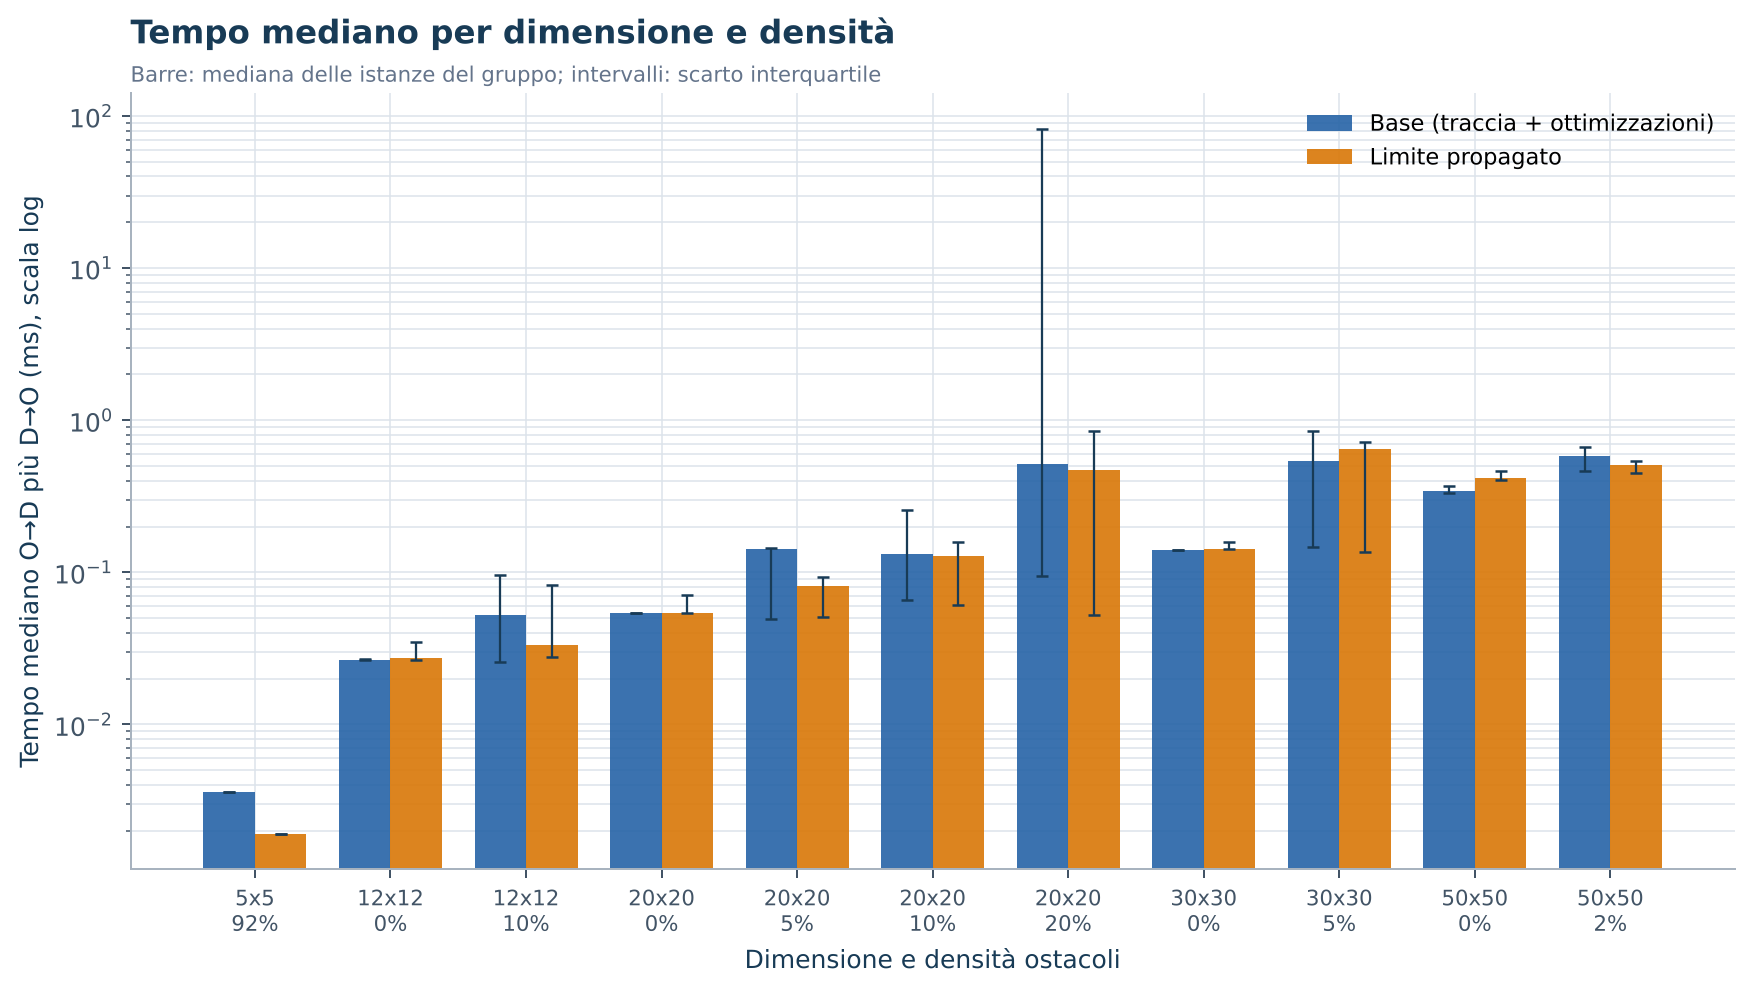
\includegraphics[width=0.92\textwidth]{grafico2_tempo_per_scenario.png}
  \caption{Tempo mediano $O \to D$ più $D \to O$ per dimensione e densità,
  varianti \code{base} e \code{limite-propagato} (scala logaritmica). Le
  barre d'errore sono l'intervallo interquartile delle istanze del gruppo.}
  \label{fig:tempo-scenario}
\end{figure}

Dalla tabella e dalla \cref{fig:tempo-scenario} emergono tre aspetti.

\begin{itemize}
  \item \textbf{Senza ostacoli il tempo cresce con la dimensione.} In tutte
        le 12 istanze senza ostacoli $D$ è nella chiusura di $O$ e basta una
        chiamata per verso. Il tempo della variante \code{base} sale da
        \num{0.027} ms a $12\times12$ a \num{0.34} ms a $50\times50$: le
        celle aumentano di 17 volte e il tempo di 13, come atteso da un
        calcolo di chiusura di costo $\Theta(n)$. Il passaggio di
        riscaldamento evita che la prima griglia misurata risulti più lenta
        di griglie più grandi a causa della compilazione JIT.
  \item \textbf{Il costo dipende dalle chiamate più che dalla dimensione.}
        Il gruppo più costoso per la variante \code{base} non è il
        $50\times50$ ma il $20\times20$ con il 20\% di ostacoli, dove una
        singola istanza richiede \num{102202} chiamate e \num{399} ms, circa
        due terzi del tempo della variante \code{base} sull'intero piano. Le
        istanze di uno stesso gruppo differiscono fino a quattro ordini di
        grandezza, perché la disposizione degli ostacoli e la posizione di
        $O$ e $D$ decidono quanti rami sopravvivono alla potatura.
  \item \textbf{Il limite propagato elimina le code.} Le mediane delle due
        varianti sono simili, perché la maggior parte delle istanze è facile
        per entrambe; il massimo del gruppo $20\times20$ al 20\% scende però
        da \num{399} ms a \num{2.1} ms e da \num{102202} a 719 chiamate.
\end{itemize}

\begin{figure}[H]
  \centering
  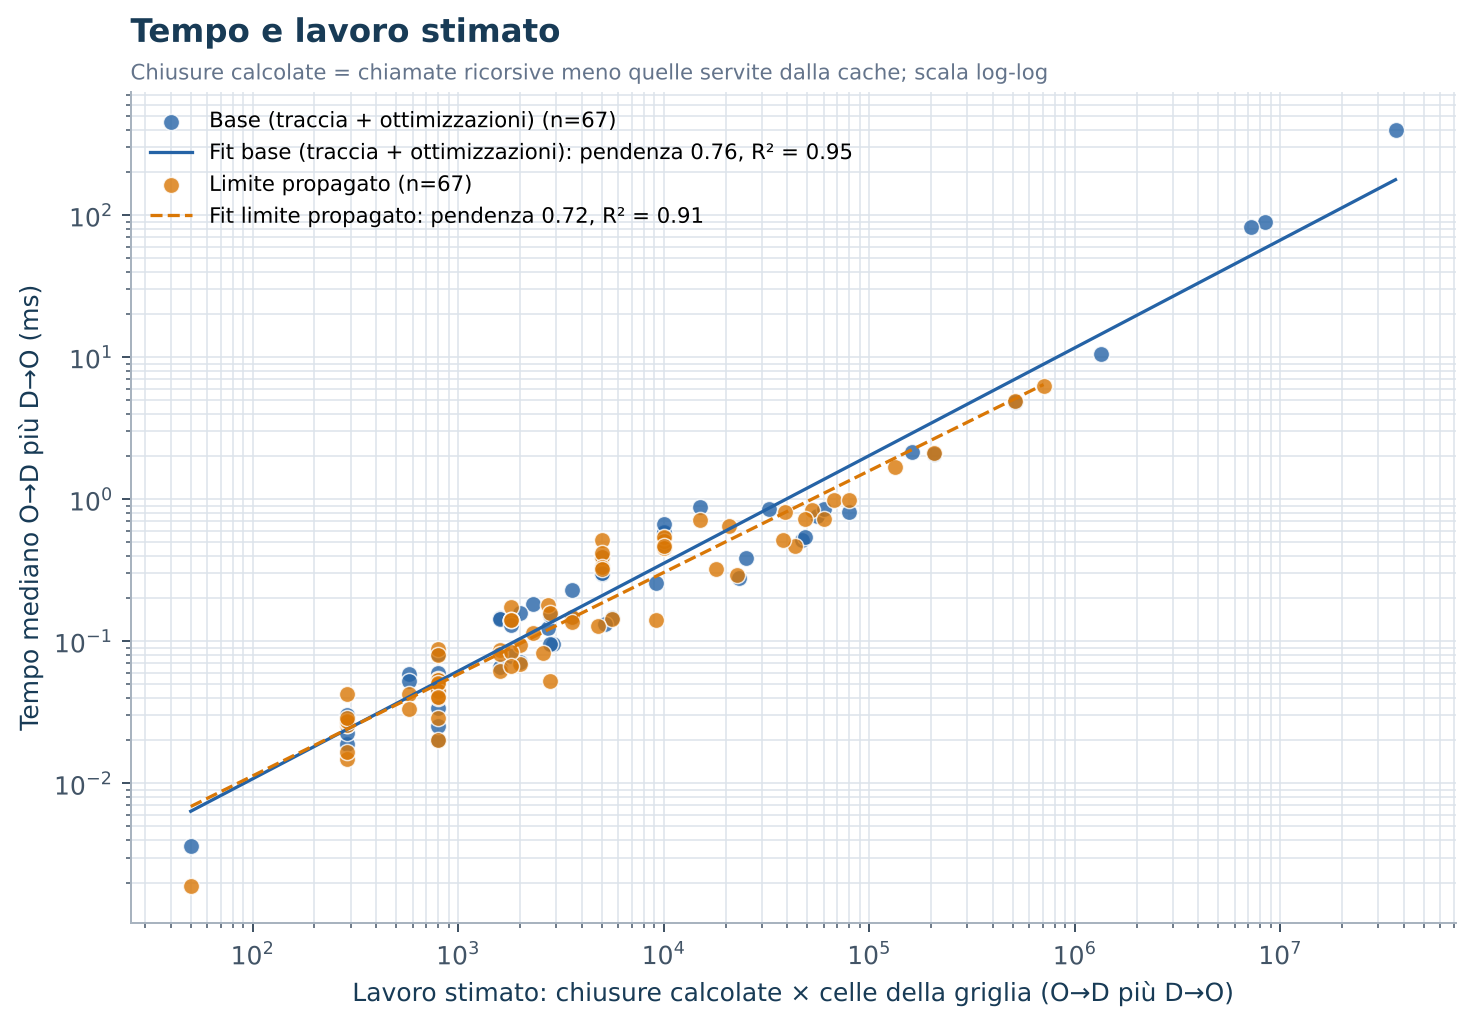
\includegraphics[width=0.82\textwidth]{grafico1_lavoro_vs_tempo.png}
  \caption{Tempo mediano rispetto al lavoro stimato $C_c \cdot n$ per le 67
  istanze, varianti \code{base} e \code{limite-propagato}, in scala log-log,
  con le rette di regressione.}
  \label{fig:lavoro-tempo}
\end{figure}

\paragraph{Che cosa determina il tempo.} La \cref{tab:predittori} confronta
quattro grandezze come predittori del tempo della variante \code{base}. Il
numero di chiamate da solo spiega il tempo in modo moderato, perché le
chiamate servite dalla cache costano poco e perché lo stesso numero di
chiusure costa di più su una griglia più grande. Il lavoro stimato
$C_c \cdot n$ della \cref{eq:tempo}, cioè le chiusure effettivamente
calcolate moltiplicate per le celle, spiega invece il 95\% della varianza
dei logaritmi (\cref{fig:lavoro-tempo}); la relazione vale anche per il
limite propagato ($R^2 = \num{0.909}$, $\rho = \num{0.955}$). La pendenza
minore di 1 indica che sulle istanze più piccole pesano costi fissi, come
l'allocazione dei risultati e le misure stesse, che non crescono con il
lavoro.

\begin{table}[H]
\centering
\small
\begin{tabular}{@{}l r r r r@{}}
\toprule
\textbf{Predittore} & \textbf{Istanze} & \textbf{Spearman $\rho$} & \textbf{Pendenza log-log} & $\mathbf{R^2}$ \\
\midrule
chiamate ricorsive $C$             & 67 & \num{0.737} & \num{0.704} & \num{0.753} \\
chiusure calcolate $C_c$           & 67 & \num{0.740} & \num{0.737} & \num{0.767} \\
celle di frontiera visitate        & 54 & \num{0.905} & \num{1.260} & \num{0.901} \\
lavoro stimato $C_c \cdot n$       & 67 & \num{0.957} & \num{0.759} & \num{0.953} \\
\bottomrule
\end{tabular}
\caption{Grandezze che spiegano il tempo mediano della variante \code{base};
per la frontiera si escludono le 13 istanze in cui è vuota. Le tre coppie di
una stessa griglia non sono osservazioni indipendenti: i valori descrivono
il piano e non permettono inferenze generali.}
\label{tab:predittori}
\end{table}

\paragraph{Potatura.} Sull'intero piano, con la variante \code{base}, la
condizione della riga 16 è risultata falsa \num{3423} volte; in altri
\num{20483} casi la riga 16 era vera e il ramo è stato potato dalla
condizione più forte della riga 17. Il dato descrive l'esecuzione con
entrambe le condizioni attive e non equivale al confronto fra le due
condizioni, che richiederebbe di eseguire l'algoritmo con la sola riga 16.

\begin{figure}[H]
  \centering
  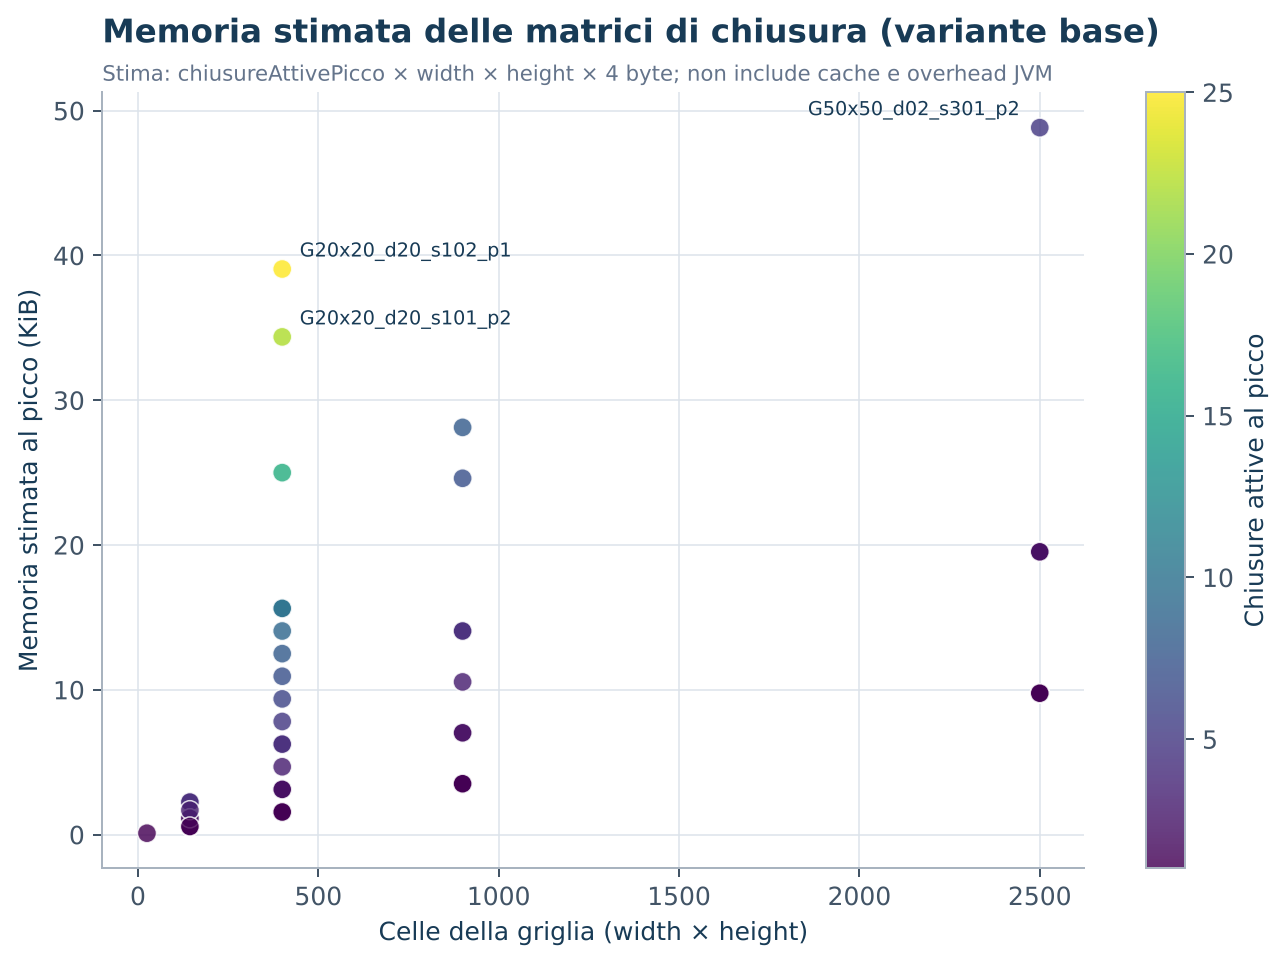
\includegraphics[width=0.75\textwidth]{grafico5_memoria_e_profondita.png}
  \caption{Memoria stimata delle matrici di chiusura attive
  contemporaneamente, variante \code{base}, rispetto al numero di celle; il
  colore indica il numero di matrici.}
  \label{fig:memoria}
\end{figure}

\paragraph{Memoria.} La memoria stimata delle matrici di chiusura
(\cref{fig:memoria}) non supera mai \num{50000} byte: il massimo corrisponde a
cinque matrici della griglia $50\times50$. Nell'istanza $20\times20$ più
costosa la ricorsione raggiunge profondità 25 con 25 matrici attive
insieme, cioè $25 \cdot 400 \cdot 4 = \num{40000}$ byte. Come osservato nella
\cref{sec:analisi-teorica}, la stima non comprende la cache.

\subsection{Effetto delle ottimizzazioni}
\label{sec:ablation}

La \cref{tab:ablation} e la \cref{fig:ablation} confrontano le quattro
varianti sui gruppi del piano con ostacoli. Per ogni gruppo sono riportati
il numero totale di chiamate ricorsive e la somma dei tempi mediani delle
istanze.

\begin{table}[H]
\centering
\small
\setlength{\tabcolsep}{4.2pt}
\begin{tabular}{@{}l r r r r r r r r@{}}
\toprule
& \multicolumn{2}{c}{\textbf{base}} & \multicolumn{2}{c}{\textbf{senza-cache}} &
  \multicolumn{2}{c}{\textbf{senza-ordinamento}} & \multicolumn{2}{c}{\textbf{limite-propagato}} \\
\cmidrule(lr){2-3}\cmidrule(lr){4-5}\cmidrule(lr){6-7}\cmidrule(l){8-9}
\textbf{Gruppo} & \textbf{chiamate} & \textbf{ms} & \textbf{chiamate} & \textbf{ms} &
  \textbf{chiamate} & \textbf{ms} & \textbf{chiamate} & \textbf{ms} \\
\midrule
$12\times12$, 10,4\% & 93            & \num{0.6}   & 97            & \num{0.8}    & 339        & \num{1.4}  & 88         & \num{0.5}  \\
$20\times20$, 5\%    & 189           & \num{1.6}   & 430           & \num{2.6}    & 941        & \num{5.6}  & 145        & \num{1.4}  \\
$20\times20$, 10\%   & 680           & \num{3.3}   & \num{1008}    & \num{5.0}    & \num{8397} & \num{30.1} & 365        & \num{2.0}  \\
$20\times20$, 20\%   & \num{149515}  & \num{574.7} & \num{608608}  & \num{2542.4} & ---        & ---        & \num{1608} & \num{6.0}  \\
$30\times30$, 5\%    & \num{1457}    & \num{8.5}   & \num{8707}    & \num{66.1}   & ---        & ---        & \num{1444} & \num{8.4}  \\
$50\times50$, 2\%    & 588           & \num{14.7}  & 588           & \num{14.0}   & ---        & ---        & 312        & \num{10.1} \\
\bottomrule
\end{tabular}
\caption{Chiamate ricorsive totali e somma dei tempi mediani per gruppo e
variante; --- indica una variante non eseguita nel gruppo.}
\label{tab:ablation}
\end{table}

\begin{figure}[H]
  \centering
  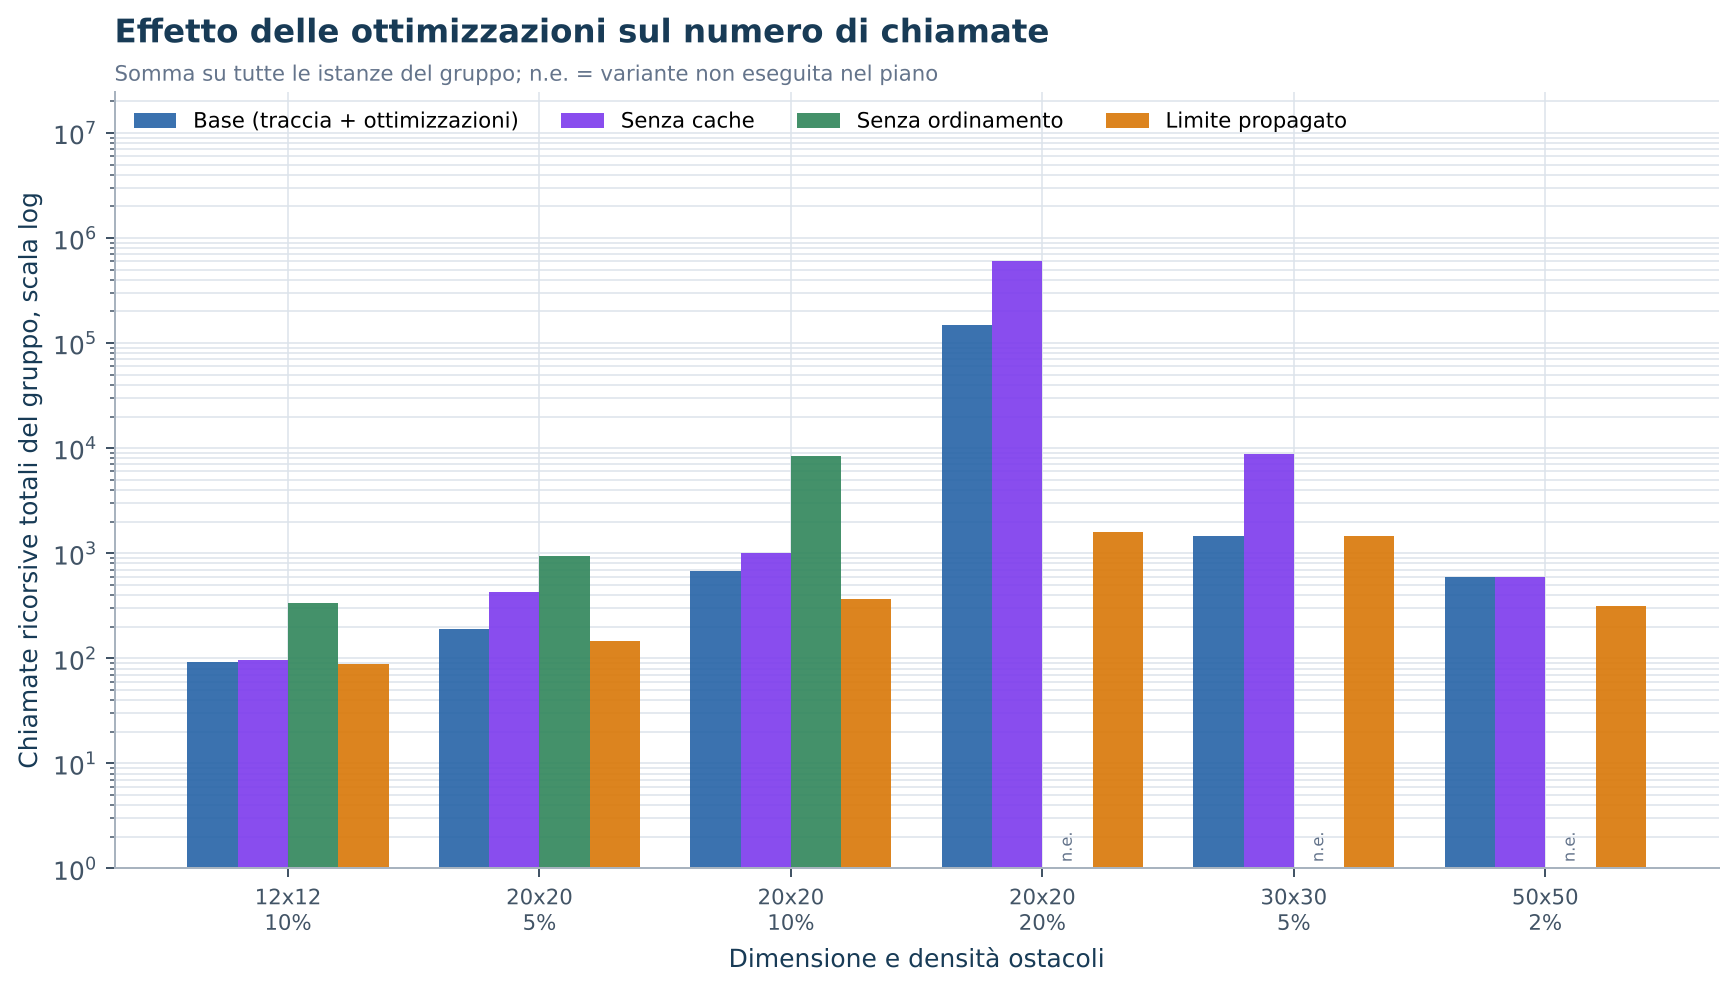
\includegraphics[width=0.92\textwidth]{grafico3_ablation.png}
  \caption{Chiamate ricorsive totali per gruppo e variante, in scala
  logaritmica.}
  \label{fig:ablation}
\end{figure}

\begin{itemize}
  \item \textbf{Ordinamento della frontiera.} È l'ottimizzazione più
        importante fra quelle della versione \code{base}: senza ordinamento le
        chiamate aumentano da 3,6 a 12 volte già sulle griglie più facili, e
        sulle griglie $20\times20$ al 20\% l'esecuzione diventa
        impraticabile. Visitando prima i candidati con limite inferiore
        minore, $\mathit{lunghezzaMin}$ scende subito e le righe 16 e 17
        potano quasi tutti gli altri rami.
  \item \textbf{Cache.} Il guadagno cresce con la difficoltà: senza cache le
        chiamate sono 4 volte tante a $20\times20$ al 20\% e 6 volte tante a
        $30\times30$ al 5\%, con tempi 4,4 e 7,8 volte maggiori. Sulle
        griglie $50\times50$ al 2\% non ci sono sottoproblemi ripetuti e la
        cache non cambia nulla.
  \item \textbf{Limite propagato.} Sull'intero piano riduce le chiamate da
        \num{152548} a \num{3988}; nel gruppo $20\times20$ al 20\% le riduce
        di 93 volte e il tempo di 96 volte. Sui gruppi in cui la versione
        \code{base} trova subito il cammino migliore il guadagno è piccolo o
        nullo, come a $30\times30$ al 5\%.
\end{itemize}

\subsection{Limiti di scala}
\label{sec:limiti-scala}

Il piano principale arriva a $50\times50$ con il 2\% di ostacoli. Per capire
dove l'algoritmo smette di essere utilizzabile, la classe \code{LimitiScala}
esegue una serie separata, salvata in \code{risultati/limiti\_scala.csv},
per le varianti \code{base} e \code{limite-propagato}:

\begin{itemize}
  \item griglie quadrate di lato 20, 30, 40, 50, 70 e 100;
  \item densità di ostacoli 0, 5, 10, 15, 20 e 30\%;
  \item tre seed (1, 2, 3) per combinazione, per un totale di 108 coppie per
        variante;
  \item $O$ nella cella libera più vicina al 10\% della diagonale e $D$ in
        quella più vicina al 90\%;
  \item ogni verso eseguito in una JVM separata con limite di \textbf{10 s}
        e memoria massima di \textbf{1 GB}; $D \to O$ viene eseguito solo se
        $O \to D$ è terminato.
\end{itemize}

Il processo separato permette di registrare un superamento del limite di
tempo (\code{TIMEOUT}) o un \code{OutOfMemoryError} (\code{OOM}) e passare
alla coppia successiva senza aggiungere a \cmin{} un meccanismo di
interruzione, che per questa versione non è richiesto. Ogni verso è una
singola esecuzione senza riscaldamento: i tempi comprendono l'avvio della
JVM e la compilazione JIT e non sono confrontabili con quelli del piano. La
serie è stata eseguita l'8 novembre 2026 sulla stessa macchina del piano, in
circa 18 minuti.

\begin{table}[H]
\centering
\small
\begin{tabular}{@{}l c c c c c c@{}}
\toprule
\textbf{Dimensione} & \textbf{0\%} & \textbf{5\%} & \textbf{10\%} & \textbf{15\%} & \textbf{20\%} & \textbf{30\%} \\
\midrule
$20\times20$   & 3 \;|\; 3 & 3 \;|\; 3 & 3 \;|\; 3 & 3 \;|\; 3 & 3 \;|\; 3 & 3 \;|\; 3 \\
$30\times30$   & 3 \;|\; 3 & 3 \;|\; 3 & 2 \;|\; 3 & 1 \;|\; 3 & 0 \;|\; 3 & 0 \;|\; 3 \\
$40\times40$   & 3 \;|\; 3 & 3 \;|\; 3 & 1 \;|\; 3 & 0 \;|\; 0 & 0 \;|\; 2 & 0 \;|\; 2 \\
$50\times50$   & 3 \;|\; 3 & 2 \;|\; 2 & 0 \;|\; 2 & 0 \;|\; 2 & 0 \;|\; 1 & 0 \;|\; 1 \\
$70\times70$   & 3 \;|\; 3 & 0 \;|\; 1 & 0 \;|\; 3 & 0 \;|\; 0 & 0 \;|\; 1 & 0 \;|\; 0 \\
$100\times100$ & 3 \;|\; 3 & 1 \;|\; 2 & 0 \;|\; 0 & 0 \;|\; 0 & 0 \;|\; 0 & 0 \;|\; 0 \\
\midrule
\textbf{Totale} & \multicolumn{6}{c}{\textbf{46} su 108 \;|\; \textbf{73} su 108} \\
\bottomrule
\end{tabular}
\caption{Coppie completate in entrambi i versi entro i limiti, su 3 per
cella: \code{base} a sinistra, \code{limite-propagato} a destra.}
\label{tab:limiti}
\end{table}

\begin{figure}[H]
  \centering
  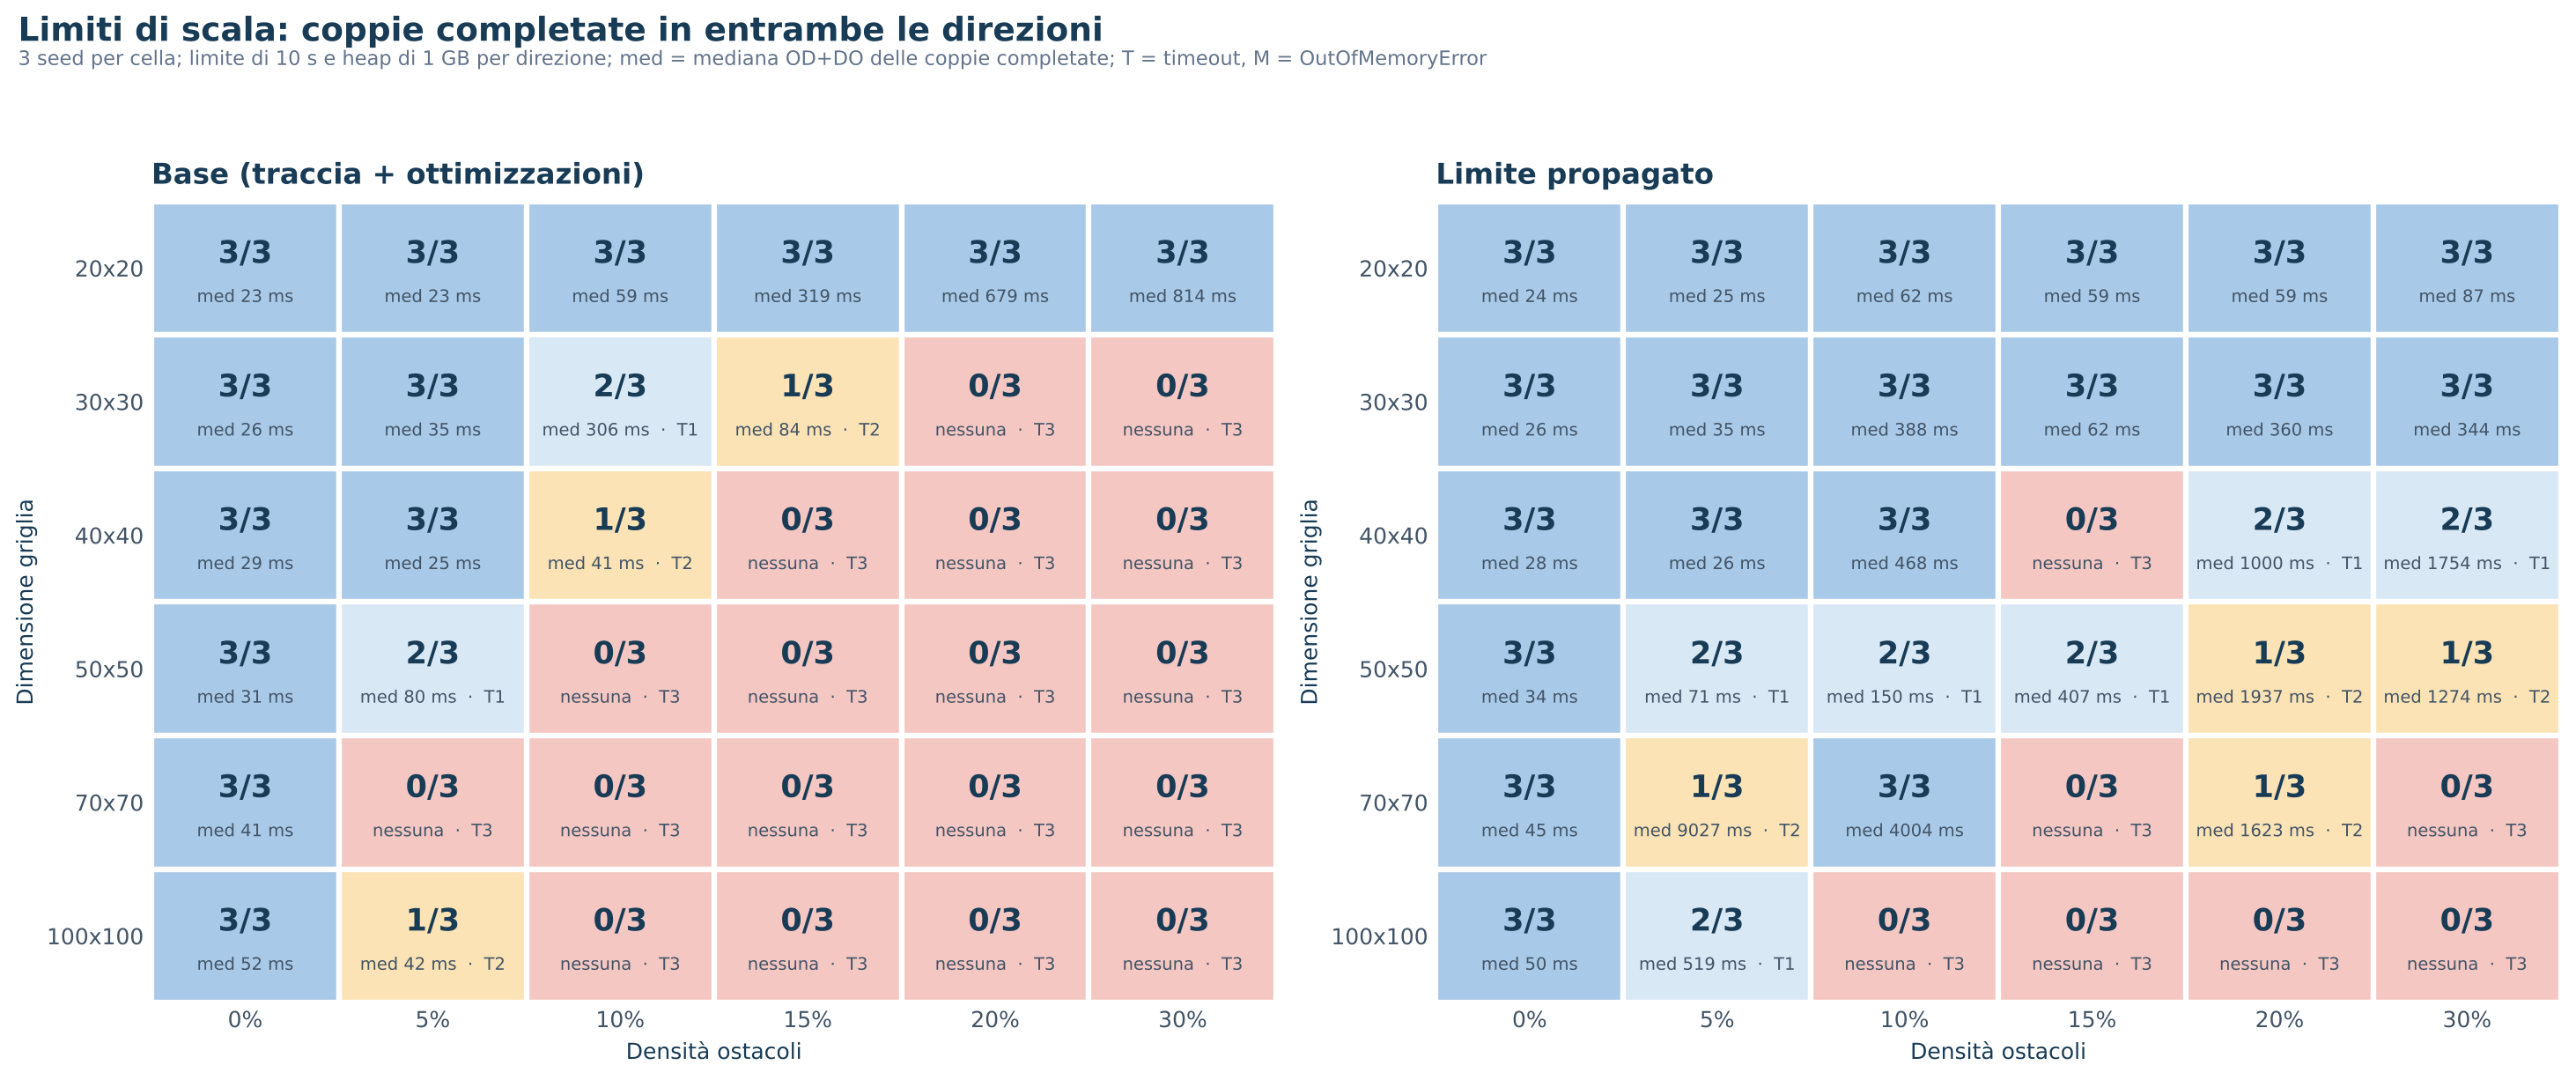
\includegraphics[width=\textwidth]{grafico6_limiti_scala.png}
  \caption{Esito della serie sui limiti di scala per le due varianti. In ogni
  cella: coppie completate, mediana del tempo $O \to D$ più $D \to O$ delle
  coppie completate e numero di esecuzioni fermate per tempo (T) o per
  memoria (M).}
  \label{fig:limiti}
\end{figure}

Con la variante \code{base} sono state completate 46 coppie su 108: le altre
62 si sono fermate per il limite di tempo già nel verso $O \to D$. Con il
limite propagato le coppie completate sono 73: le stesse 46 più altre 27,
mentre 34 si sono fermate nel verso $O \to D$ e una nel verso $D \to O$,
sempre per il limite di tempo. Nessuna esecuzione ha esaurito la memoria.
Tutte le coppie completate sono simmetriche e, dove entrambe le varianti
terminano, le lunghezze coincidono. Numero di chiamate e lunghezze non
dipendono dalla macchina; su hardware diverso possono cambiare esito solo le
coppie che terminano vicino ai 10 s.

Dalla serie emergono cinque osservazioni.

\begin{enumerate}
  \item \textbf{Senza ostacoli la dimensione non è un problema.} Le 18 coppie
        allo 0\% terminano con una sola chiamata per verso, perché in assenza
        di ostacoli ogni cella della griglia appartiene al contesto di $O$. I
        tempi, fra 23 e 52 ms anche a $100\times100$, sono quelli di un
        calcolo di chiusura con la JVM appena avviata.
  \item \textbf{Per la variante \code{base} il fattore critico è la
        densità.} A $20\times20$ tutte le densità sono gestibili, ma la
        mediana passa da 23 ms allo 0\% a 814 ms al 30\%. A $30\times30$ si
        perdono coppie dal 10\% in su, a $50\times50$ resta parzialmente
        gestibile solo il 5\%, a $70\times70$ e $100\times100$ nessuna
        densità diversa da zero è gestibile in modo affidabile.
  \item \textbf{Il limite propagato sposta il confine.} Completa tutte le
        coppie $30\times30$ fino al 30\% e più della metà di quelle
        $40\times40$ e $50\times50$ con ostacoli. Sulle 46 coppie completate da entrambe le varianti,
        le chiamate del verso $O \to D$ scendono da \num{1096774} a
        \num{20140}. La coppia più costosa per la variante \code{base}
        ($20\times20$, 30\%, seed 1) richiede \num{480274} chiamate,
        profondità 24, \num{2.1} s e fino a 390 MB di heap; con il limite
        propagato bastano 362 chiamate, 49 ms e 9 MB.
  \item \textbf{La crescita resta combinatoria.} Anche con il limite
        propagato le griglie $70\times70$ e $100\times100$ superano quasi
        sempre i 10 s; la coppia completata più costosa ($70\times70$, 5\%,
        seed 2) richiede \num{508161} chiamate e \num{8.8} s nel solo verso
        $O \to D$. Come previsto dalla \cref{sec:analisi-teorica}, le
        ottimizzazioni riducono il numero di chiamate ma non il caso
        peggiore.
  \item \textbf{I due versi possono costare in modo molto diverso.} Per
        ciascuna variante, in 5 coppie completate un verso è più lento
        dell'altro di oltre 10 volte, per esempio \num{1410} ms contro 29 ms
        a $20\times20$ con il 15\% (seed 3, \code{base}). Una spiegazione
        plausibile è che in un verso si trovi presto un cammino corto, che
        consente di potare molti più rami.
\end{enumerate}
\clearpage
\section{Conclusioni}
\label{sec:conclusioni}

Il progetto realizza i quattro compiti nella versione per una persona. Il
generatore produce griglie casuali riproducibili e le salva in JSON. Il
calcolo della chiusura determina contesto, complemento e frontiera in una
sola passata di costo lineare nel numero di celle ed è disponibile anche da
riga di comando. \cmin{} restituisce la lunghezza del cammino minimo e la
sequenza dei landmark, oppure lunghezza infinita e sequenza vuota. La
correttezza è sostenuta dalla verifica di simmetria su tutte le esecuzioni,
dal confronto con Dijkstra di tutte le varianti su griglie casuali e su
griglie costruite per forzare ricorsioni profonde, e dall'enumerazione
completa delle griglie $3\times3$ per la chiusura.

La sperimentazione mostra che il tempo di \cmin{} è spiegato quasi del tutto
dal lavoro stimato, cioè dalle chiusure calcolate moltiplicate per le celle
della griglia. Il numero di chiusure dipende dalla densità e dalla
disposizione degli ostacoli più che dalla dimensione: senza ostacoli
l'algoritmo risolve griglie $100\times100$ in poche decine di millisecondi.
Fra le ottimizzazioni, l'ordinamento della frontiera è indispensabile e la
cache conta sulle istanze difficili. Il limite propagato riduce le chiamate
del piano da \num{152548} a \num{3988} e porta le coppie completate entro
10 s da 46 a 73 su 108, senza cambiare alcuna lunghezza; la crescita resta
però combinatoria, e a $100\times100$ dal 10\% di ostacoli in su nessuna
coppia termina entro il limite di tempo.

\subsection{Limitazioni}

\begin{itemize}
  \item \textbf{Crescita combinatoria.} Il numero di chiamate non ha un
        limite polinomiale. Con 10 s e 1 GB per verso, la variante
        \code{base} è affidabile solo fino a $20\times20$ per tutte le
        densità provate e fino a $40\times40$ con il 5\% di ostacoli; il
        limite propagato estende la zona affidabile a $30\times30$ per tutte
        le densità (\cref{sec:limiti-scala}). Il piano principale resta
        dentro questa zona e non va letto come rappresentativo di griglie
        grandi e dense.
  \item \textbf{Costo lineare per chiusura.} Il calcolo della chiusura
        scandisce sempre l'intera griglia, anche quando la chiusura contiene
        poche celle.
  \item \textbf{Memoria della cache.} La cache conserva un elemento per ogni
        sottoproblema risolto, anche quando i sottoproblemi identici sono
        rari: nel caso più costoso della variante \code{base} le chiamate
        servite dalla cache sono il 13\% del totale.
  \item \textbf{Variante senza ordinamento.} Nel piano è eseguita solo sulle
        griglie più facili, perché sulle altre richiede da secondi a decine
        di secondi per esecuzione; il suo costo sulle istanze difficili è
        quindi documentato solo in modo qualitativo.
  \item \textbf{Misure dei tempi.} Il piano usa un passaggio di
        riscaldamento, un riscaldamento per esecuzione e cinque ripetizioni,
        senza un framework come JMH; il CSV conserva minimo, mediana e
        massimo ma non le misure grezze. Le tre coppie di una stessa griglia
        non sono osservazioni indipendenti, quindi correlazioni e regressioni
        descrivono il piano e non permettono inferenze generali.
  \item \textbf{Stima della memoria.} Il campo \code{memEst} conta solo le
        matrici di chiusura; il picco di heap della serie sui limiti di scala
        è un limite superiore, non una misura esatta.
  \item \textbf{Ambiente.} Il codice è compilato per Java 17 ma è stato
        eseguito solo su JDK 21.
\end{itemize}

\subsection{Sviluppi futuri}

\begin{itemize}
  \item \textbf{Chiusura incrementale.} Limitare il calcolo alla regione
        effettivamente raggiunta, invece di scandire tutta la griglia,
        renderebbe il costo di una chiamata proporzionale alla chiusura
        invece che alla griglia; per la \cref{eq:tempo} è il fattore $n$ del
        lavoro stimato.
  \item \textbf{Cache con politica di rimozione.} Limitare la cache ai
        sottoproblemi riusati più spesso ridurrebbe la memoria sulle istanze
        con pochi riusi.
  \item \textbf{Uscita anticipata dal ciclo.} Con la frontiera ordinata per
        limite inferiore, la prima cella che viola la condizione della riga
        17 implica che la violano anche le successive: il ciclo potrebbe
        terminare lì. I rami potati non ricorrono già, quindi il guadagno
        sarebbe limitato al costo del ciclo.
  \item \textbf{Misure più robuste.} Benchmark con JMH, più ripetizioni,
        salvataggio delle misure grezze ed esecuzione anche su JDK 17.
  \item \textbf{Ricostruzione del percorso.} La sequenza delle mosse si
        ottiene percorrendo il cammino libero di ogni tratto fra landmark;
        il requisito appartiene alla versione per tre persone.
\end{itemize}
\clearpage
\section{Utilizzo del codice}
\label{sec:utilizzo}

\subsection{Contenuto della consegna}

\begin{lstlisting}
progetto_ASD/
|-- README.md
|-- pom.xml                   build Maven
|-- asd-project.jar           eseguibile precompilato
|-- requirements-report.txt   dipendenze Python per i grafici
|-- src/main/java/mio/        codice applicativo
|-- src/test/java/mio/        test JUnit
|-- risultati/
|   |-- esperimenti.csv       piano sperimentale (67 istanze, 215 righe)
|   |-- riassunti.txt         riassunto di ogni riga del piano
|   |-- limiti_scala.csv      serie sui limiti di scala (108 coppie per variante)
|   |-- griglie_json/         23 griglie del piano
|   |-- grafici/              grafici della relazione
|   `-- genera_grafici.py     script di analisi
`-- relazione/                sorgenti LaTeX e PDF di questa relazione
\end{lstlisting}

\subsection{Requisiti}

\begin{itemize}
  \item Java 17 o successivo per eseguire il JAR;
  \item Maven 3.9 o successivo per compilare ed eseguire i test;
  \item Python 3 con i pacchetti di \code{requirements-report.txt} per
        rigenerare i grafici;
  \item una distribuzione \LaTeX{} con \code{latexmk} per ricompilare la
        relazione.
\end{itemize}

\subsection{Esecuzione}

Tutti i comandi vanno eseguiti dalla radice della consegna: i file di
output sono scritti nella cartella \code{risultati/}.

\paragraph{Piano sperimentale.} Senza argomenti l'applicazione esegue il
piano della \cref{sec:protocollo}, stampa un riassunto per istanza e
variante e riscrive \code{esperimenti.csv}, \code{riassunti.txt} e le griglie
della cartella \code{griglie\_json/}. Richiede meno di un minuto.

\begin{lstlisting}
java -jar asd-project.jar
\end{lstlisting}

\paragraph{Serie sui limiti di scala.} Riscrive
\code{risultati/limiti\_scala.csv} per le varianti \code{base} e
\code{limite-propagato}. Richiede circa 18 minuti, quasi tutti dovuti alle
esecuzioni che raggiungono il limite di 10 s; indicando una variante si
esegue la serie solo per quella.

\begin{lstlisting}
java -jar asd-project.jar --limiti-scala
java -jar asd-project.jar --limiti-scala limite-propagato
\end{lstlisting}

\paragraph{Compito Due.} Calcola contesto, complemento e frontiera di $O$ e
la distanza libera fra $O$ e $D$ su una griglia salvata
(\cref{sec:applicazione-chiusura}).

\begin{lstlisting}
java -jar asd-project.jar --grid-input risultati/griglie_json/scenario_02_12x12_15ost_seed50.json --origin 0,0 --destination 10,10 --chiusura
\end{lstlisting}

\paragraph{Compito Tre, istanza singola.} Genera una griglia con i
parametri indicati, oppure la legge da un file JSON, esegue \cmin{} nei due
versi una sola volta con la variante scelta e salva il risultato. Se $O$ o
$D$ cadono su un ostacolo viene usata la cella libera più vicina e
l'applicazione lo segnala.

\begin{lstlisting}
java -jar asd-project.jar --width 20 --height 20 --obstacles 40 --seed 77 --origin 0,0 --destination 19,19 --summary true --output risultati/prova.csv --grid-output risultati/prova.json
java -jar asd-project.jar --grid-input risultati/prova.json --origin 0,0 --destination 19,19 --variante limite-propagato
\end{lstlisting}

\begin{table}[H]
\centering
\small
\begin{tabularx}{\textwidth}{@{}l X@{}}
\toprule
\textbf{Opzione} & \textbf{Significato e valore predefinito} \\
\midrule
\code{-{}-width N}, \code{-{}-height N} & dimensioni della griglia generata (20 e 20) \\
\code{-{}-obstacles N}   & numero di ostacoli, da 0 a $WH-1$ (20) \\
\code{-{}-seed N}        & seed del generatore (42) \\
\code{-{}-grid-input f.json} & griglia letta da file invece che generata;
                           esclude le quattro opzioni precedenti e
                           \code{-{}-grid-output}; nel CSV il seed vale $-1$ \\
\code{-{}-origin x,y}    & origine $O$ (\code{0,0}) \\
\code{-{}-destination x,y} & destinazione $D$ (angolo opposto all'origine) \\
\code{-{}-chiusura}      & esegue solo il Compito Due: mappa della chiusura di $O$,
                           conteggi e $\dlib(O,D)$ \\
\code{-{}-chiusura-output f.json} & con \code{-{}-chiusura}, salva gli stati delle celle \\
\code{-{}-variante v}    & variante di \cmin{}: \code{base} (predefinita),
                           \code{senza-cache}, \code{senza-ordinamento},
                           \code{limite-propagato} \\
\code{-{}-summary true|false} & stampa del riassunto (\code{true}) \\
\code{-{}-output f.csv}  & CSV del risultato (\code{risultati/esperimento\_personalizzato.csv}) \\
\code{-{}-grid-output f.json} & griglia generata (\code{risultati/griglie\_json/personalizzata.json}) \\
\code{-{}-limiti-scala [v]} & serie sui limiti di scala, per entrambe le
                           varianti principali o solo per $v$; va usata da sola \\
\code{-{}-help}          & elenco delle opzioni \\
\bottomrule
\end{tabularx}
\caption{Opzioni della riga di comando.}
\label{tab:opzioni}
\end{table}

\subsection{Compilazione e test}

\begin{lstlisting}
mvn -q clean package
java -jar target/asd-project-1.0-SNAPSHOT.jar
\end{lstlisting}

Il primo comando compila il codice, esegue i 68 test e crea in
\code{target/} un JAR equivalente a \code{asd-project.jar}. Per eseguire
solo i test si usa \code{mvn -q test}.

\subsection{Grafici e relazione}

\begin{lstlisting}
python -m pip install -r requirements-report.txt
python risultati/genera_grafici.py
cd relazione
latexmk -pdf Relazione_ASD_2024_25.tex
\end{lstlisting}

Lo script dei grafici verifica la struttura dei due file CSV e la coerenza
delle lunghezze fra varianti prima di disegnare, scrive le immagini in
\code{risultati/grafici/}, da cui la relazione le include direttamente, e
stampa i valori riassuntivi riportati nella \cref{sec:compito4}.
\clearpage

\appendix
\section{Formato dei file di output}
\label{app:formato}

\subsection{\code{esperimenti.csv}}

Una riga per istanza e variante, 31 colonne, decimali con il punto. Le sequenze dei
landmark sono racchiuse fra virgolette perché contengono virgole; una
lunghezza infinita è scritta \code{INF} e la relativa sequenza \code{[]}.

\begin{table}[H]
\centering
\small
\begin{tabularx}{\textwidth}{@{}>{\raggedright\arraybackslash}p{6.1cm} X@{}}
\toprule
\textbf{Colonne} & \textbf{Significato} \\
\midrule
\code{gridId} & identificativo dell'istanza, per esempio
  \code{G12x12\_d10\_s50\_p1} (dimensioni, densità in percentuale, seed,
  numero della coppia) \\
\code{variante} & variante di \cmin{} (\cref{tab:varianti}) \\
\code{tipoGriglia} & tipo di griglia, sempre \code{Casuale} \\
\code{width}, \code{height}, \code{nOstacoli}, \code{seed} & parametri della griglia \\
\code{Ox}, \code{Oy}, \code{Dx}, \code{Dy} & coordinate effettive di $O$ e $D$ \\
\code{lunghezzaOD}, \code{lunghezzaDO} & lunghezze nei due versi, 6 decimali \\
\code{sequenzaLandmarkOD}, \code{sequenzaLandmarkDO} & sequenze dei landmark,
  ogni elemento nella forma \code{(x=..,y=..,tipo=..)} \\
\code{correttezza} & esito della verifica di simmetria \\
\code{frontieraTot} & celle di frontiera di tutte le chiusure calcolate \\
\code{falsiRiga16} & volte in cui la riga 16 è risultata falsa \\
\code{falsiRiga17} & potature dovute alla sola riga 17 \\
\code{pruningTotale} & somma delle due precedenti \\
\code{chiamateRicorsive}, \code{cacheHit} & invocazioni totali e invocazioni
  servite dalla cache \\
\code{profonditaMassima} & profondità massima della ricorsione \\
\code{chiusureAttivePicco} & matrici di chiusura attive
  contemporaneamente lungo la pila delle chiamate, al picco \\
\code{celleChiusuraTotali} & somma delle dimensioni delle chiusure calcolate \\
\code{memoriaMatriciPiccoBytesStimata} & $\code{chiusureAttivePicco} \cdot
  W \cdot H \cdot 4$ byte \\
\code{warmupEseguiti}, \code{ripetizioniTempo} & riscaldamenti e ripetizioni
  misurate \\
\code{tempoMinNs}, \code{tempoMedianoNs}, \code{tempoMaxNs} & tempi delle
  ripetizioni in nanosecondi, versi $O \to D$ e $D \to O$ insieme \\
\bottomrule
\end{tabularx}
\caption{Colonne di \code{esperimenti.csv}. Tutti i contatori sommano i due
versi.}
\end{table}

\subsection{\code{limiti\_scala.csv}}

Una riga per variante e coppia, 24 colonne.

\begin{table}[H]
\centering
\small
\begin{tabularx}{\textwidth}{@{}>{\raggedright\arraybackslash}p{6.1cm} X@{}}
\toprule
\textbf{Colonne} & \textbf{Significato} \\
\midrule
\code{variante} & \code{base} oppure \code{limite-propagato} \\
\code{width}, \code{height}, \code{densitaPerc}, \code{nOstacoli}, \code{seed}
  & parametri della griglia \\
\code{Ox}, \code{Oy}, \code{Dx}, \code{Dy} & coordinate di $O$ e $D$ \\
\code{esitoOD}, \code{esitoDO} & \code{OK}, \code{TIMEOUT}, \code{OOM},
  \code{STACK} o \code{ERRORE}; \code{esitoDO} vale \code{NON\_ESEGUITO} se
  il verso $O \to D$ non è terminato \\
\code{lunghezzaOD}, \code{lunghezzaDO} & lunghezze, \code{INF} o vuote se il
  verso non è terminato \\
\code{simmetria} & \code{true} o \code{false} se entrambi i versi sono
  terminati, altrimenti \code{ND} \\
\code{tempoODms}, \code{tempoDOms} & tempo di una singola esecuzione a
  freddo, in millisecondi \\
\code{chiamateOD}, \code{profonditaOD}, \code{frontieraOD}, \code{cacheHitOD}
  & contatori del verso $O \to D$ \\
\code{piccoHeapMBOD} & somma dei picchi delle aree di heap della JVM, in MB \\
\code{timeoutMs}, \code{heapMax} & limiti applicati a ogni verso \\
\bottomrule
\end{tabularx}
\caption{Colonne di \code{limiti\_scala.csv}.}
\end{table}

\subsection{\code{riassunti.txt}}

Una riga per ogni riga di \code{esperimenti.csv}, nel formato del riassunto
della \cref{sec:contatori}, nello stesso ordine del CSV.

\subsection{Griglie JSON}

Ogni file di \code{risultati/griglie\_json/} contiene un array di righe;
ogni elemento è lo stato della cella secondo la \cref{tab:statocella}
($0$ libera, $128$ ostacolo). Il nome del file riporta numero dello scenario,
dimensioni, ostacoli e seed, per esempio
\code{scenario\_02\_12x12\_15ost\_seed50.json}.


\clearpage
\begin{thebibliography}{9}
\bibitem{traccia}
M.~Zanella, \emph{Progetto di Algoritmi e Strutture Dati, A.A.\ 2024/25}, testo dell'elaborato, Università degli Studi di Brescia.

\bibitem{dijkstra}
E.~W.~Dijkstra, \emph{A note on two problems in connexion with graphs}, Numerische Mathematik, 1:269--271, 1959.

\bibitem{random}
Oracle, \emph{Java SE 17 API: \code{java.util.Random}},
\url{https://docs.oracle.com/en/java/javase/17/docs/api/java.base/java/util/Random.html}.

\bibitem{bitset}
Oracle, \emph{Java SE 17 API: \code{java.util.BitSet}},
\url{https://docs.oracle.com/en/java/javase/17/docs/api/java.base/java/util/BitSet.html}.

\bibitem{jmh}
OpenJDK, \emph{Java Microbenchmark Harness (JMH)},
\url{https://github.com/openjdk/jmh}.
\end{thebibliography}

\end{document}
